\part{Guide Utilisateur}

\chapter{Navigation sans connexion}

Cette partie décrit les 3 pages accessibles par un utilisateur non connecté.

\section{La page d'accueil}

\subsection{Le carrousel}

Sur la page d'accueil, vous trouverez des photos des anciens tournois qui
défilent automatiquement. Vous pouvez également cliquer à droite ou à gauche
de ces images si vous souhaitez les revoir sans attendre un tour complet de
toutes les photos. \newline

\subsection{Le décompte}

Un décompte s'affiche sur votre écran. Il correspond à l'attente qu'il reste
jusqu'au début du prochain tournoi organisé par Le Charles de Lorraine. Une
fois que le décompte sera terminé, vous pourrez accéder à une page qui
présentera les résultats du tournoi en cours. \newline

\subsection{La description}

Cette partie vous permet d'en savoir plus sur l'histoire du tournoi et vous
propose un lien pour avoir accès aux résultats des éditions précédentes.

\subsection{Les sponsors}

Le Charles de Lorraine souhaitent remercier les sponsors qui permettent
l'organisation du tournoi dans les meilleures conditions. Ceux-ci sont vitaux
pour l'association. Si vous souhaitez devenir un sponsor du Charles de Lorraine,
n'hésitez pas à nous envoyer un mail via notre formulaire de contact.
% TODO
\todo[inline]{Ajouter une référence vers la page de contact}


\section{La page des sponsors}

\subsection{Les sponsors}


\section{Page de contact}

\begin{figure}[H]
\centering
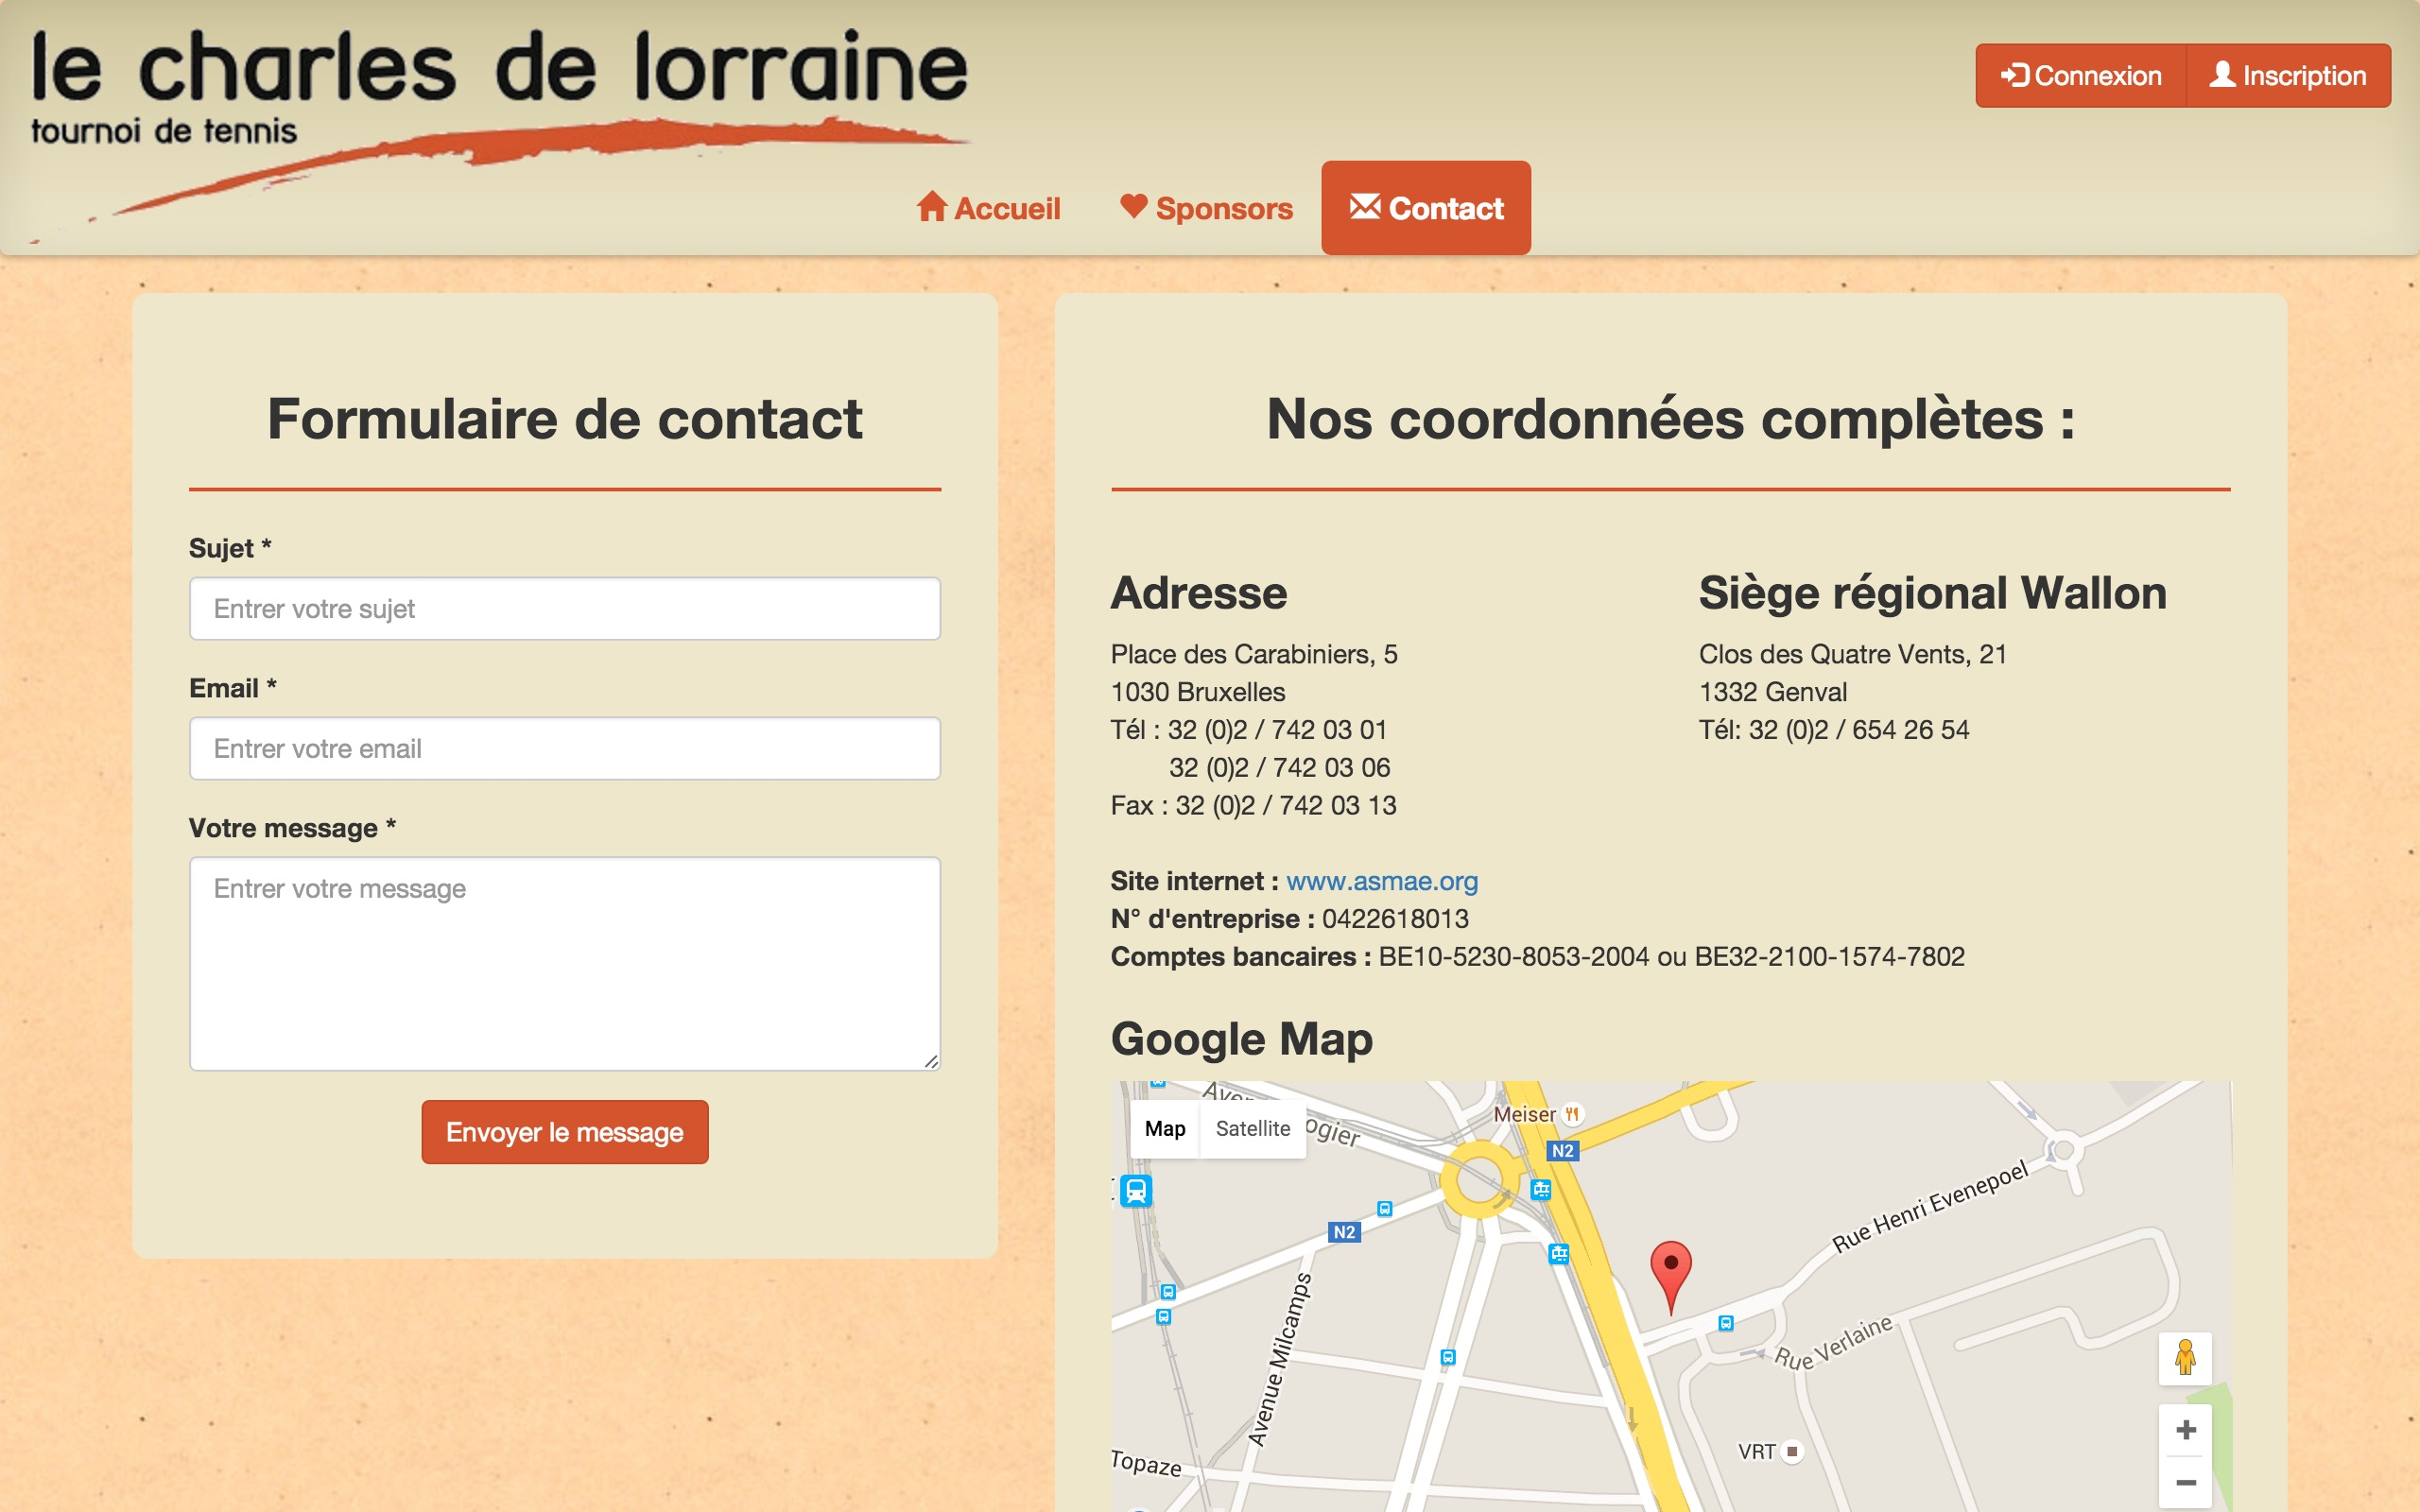
\includegraphics[scale=0.15]{page-contact/page-contact.jpg}
\caption{Page de contact}
\end{figure}

La page de contact est la troisième page accessible lorsque vous vous connectez au site web. Cette page permet de nous contacter ou de vous informer de nos coordonnées.

\subsection{Formulaire de contact}

En remplissant le formulaire et en appuyant sur le bouton \textit{Envoyer le
message}, un mail nous sera envoyé et nous vous répondrons dans les plus brefs
délais. Entrez une adresse mail valide et tentez d'être le plus complet
possible dans votre message afin que nos échanges soient les plus efficaces
possibles.

\begin{figure}[H]
\centering
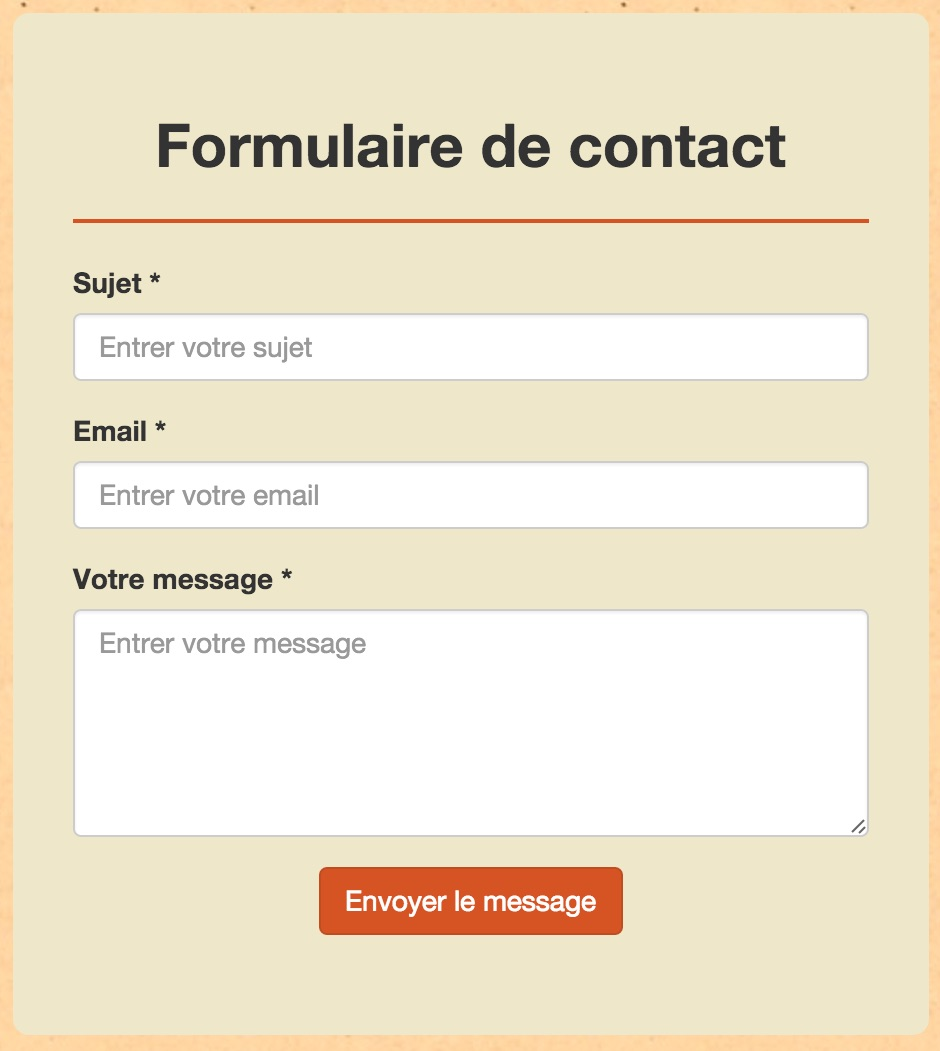
\includegraphics[scale=0.15]{page-contact/page-contact-formulaire.jpg}
\caption{Page de contact - le formulaire de contact}
\end{figure}

\subsection{Les coordonnées de ASMAE}

Ces coordonnées vous permettent de nous contacter par d'autres voies que les
emails. L'équipe du \textit{Charles de Lorraine} sera ravie de vous répondre quelque
soit votre demande liée au tournoi.

\begin{figure}[H]
\centering
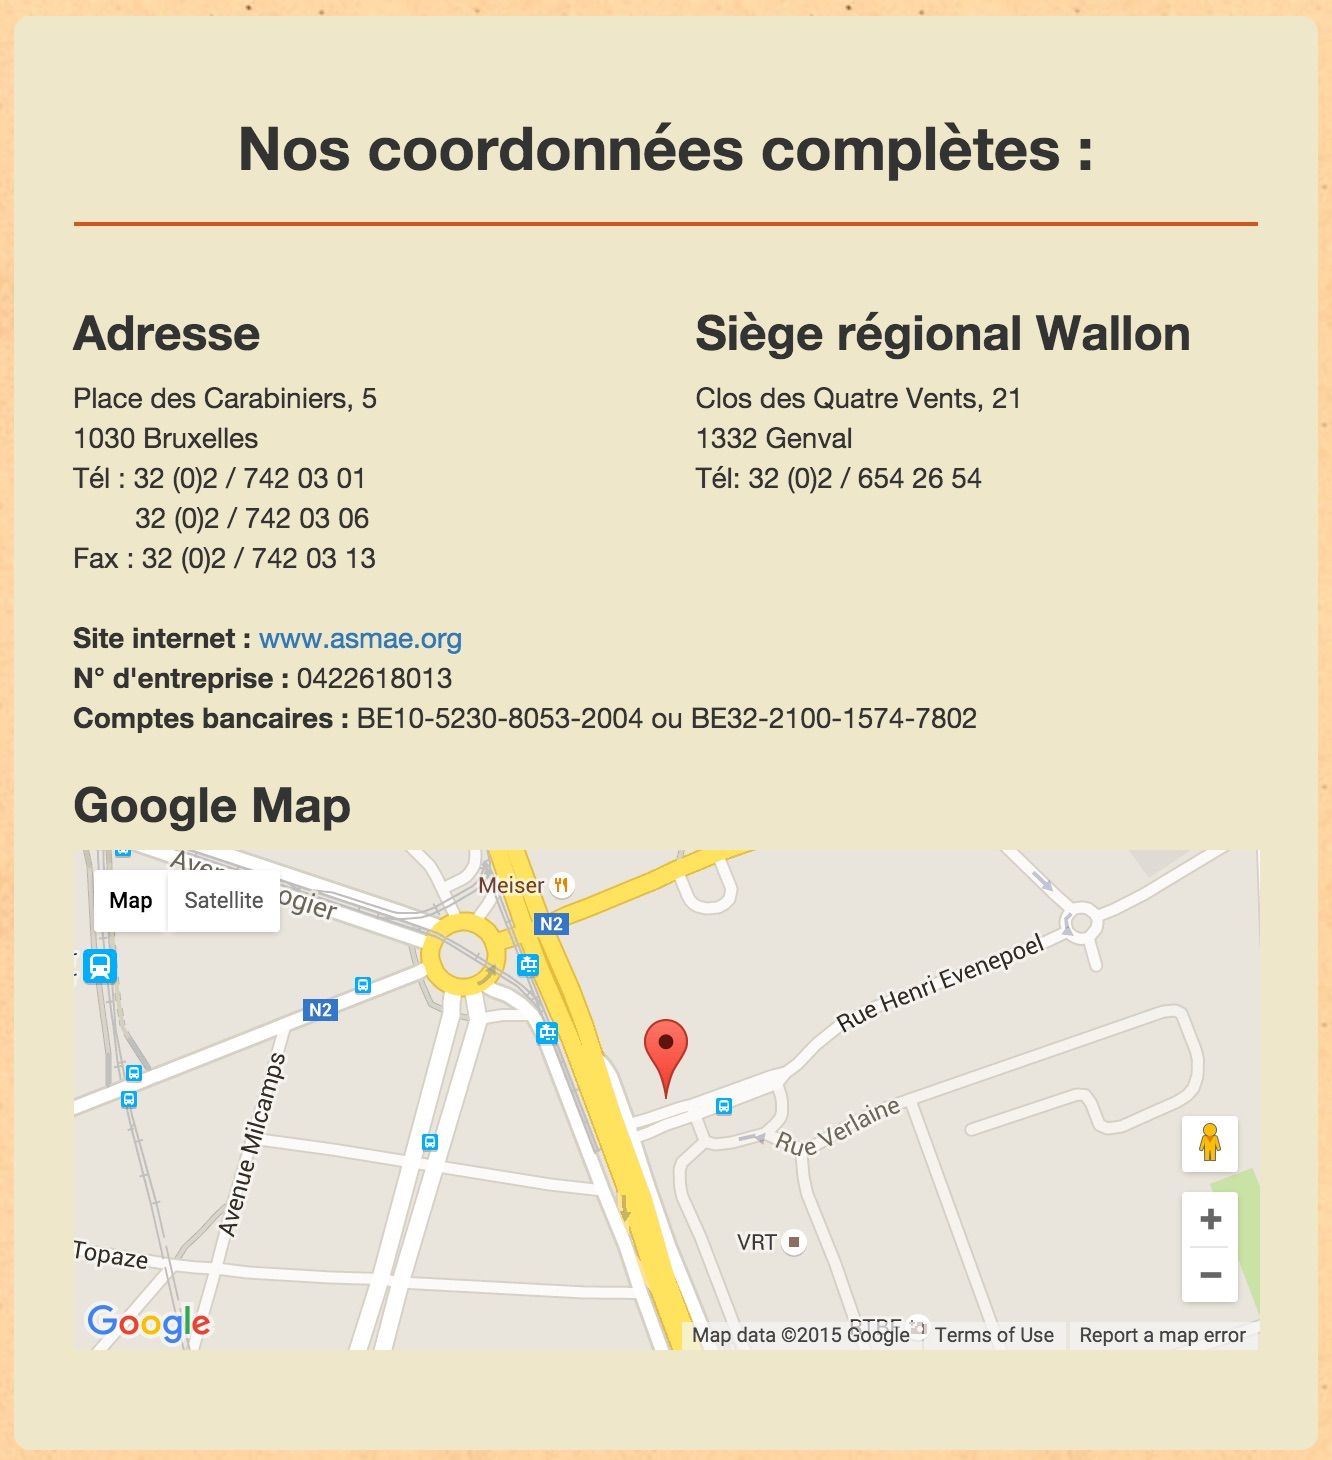
\includegraphics[scale=0.15]{page-contact/page-contact-coordonnees.jpg}
\caption{Page de contact - les coordonnées de ASMAE.}
\end{figure}


\chapter{Utilisateur standard}

Cette partie est adressé à tous les utilisateurs souhaitant participer à l'événement, que ce soit en tant que joueurs ou en tant que propriétaire d'un terrain. \newline

La première catégorie décrit les fonctionnalités liées à un compte, la deuxième concerne l'inscription à un tournoi, et la troisième concerne la gestion des terrains (pour les propriétaires de terrains).

\section{Compte}

Dans cette section, il est expliqué comment créer un compte, gérer ce compte, et se connecter, et se déconnecter.

\subsection{Créer un compte}

Pour créer un compte utilisateur à partir de n'importe quelle page, cliquez sur le bouton "Inscription" proposé dans le menu spécial dans le coin en haut, à droite de l'écran, comme indiqué à la figure ci-dessous.

\begin{figure}[H]
\centering
\includegraphics[scale=0.15]{user_images/basic_user/GererConnexion/Senregistrer/001.jpg}
\caption{Création compte, étape 1}
\end{figure}

Ensuite, remplissez le formulaire pour créer un compte. Celui-ci est décomposé en 2 parties : la première concerne les informations importantes de connexion, et la deuxième partie concerne les informations personnelles de l'utilisateur. \newline

Les champs dont le nom est suivi par une étoile (*) doivent obligatoirement être remplis. Les autres champs sont optionnels.

\begin{figure}[H]
\centering
\includegraphics[scale=0.15]{user_images/basic_user/GererConnexion/Senregistrer/002.jpg}
\caption{Création compte, étape 2}
\end{figure}

Lorsque vous avez terminé de remplir le formulaire, vous pouvez cliquer sur le bouton "Inscription" en bas de la page, comme indiqué à la figure ci-dessous.

\begin{figure}[H]
\centering
\includegraphics[scale=0.15]{user_images/basic_user/GererConnexion/Senregistrer/003.jpg}
\caption{Création compte, étape 3}
\end{figure}

Si le formulaire est invalide, vous aurez un message indiquant précisément l'erreur. Dans le cas contraire, vous serez invités à consulter vos emails à l'adresse email que vous avez mis dans le formulaire, comme le montre l'image ci-dessous.

\begin{figure}[H]
\centering
\includegraphics[scale=0.15]{user_images/basic_user/GererConnexion/Senregistrer/004.jpg}
\caption{Création compte, étape 4}
\end{figure}

Vous pouvez accéder à la plupart des pages d'un utilisateur standard. Pour accéder pleinement à toutes les pages d'un utilisateur standard, vous devez obligatoirement valider votre adresse email. \newline

Dans votre boîte email, vous devriez avoir un email similaire à celui sur l'image ci-dessous. Un lien vous est proposé pour valider votre compte.

\begin{figure}[H]
\centering
\includegraphics[scale=0.20]{user_images/basic_user/GererConnexion/Senregistrer/005.jpg}
\caption{Création compte, étape 5}
\end{figure}

Si vous cliquez sur le lien, ou copiez-collez le lien dans la barre de navigation de votre navigateur web, vous accéderez à une page qui vous confirme la validation de votre adresse email.

\begin{figure}[H]
\centering
\includegraphics[scale=0.15]{user_images/basic_user/GererConnexion/Senregistrer/006.jpg}
\caption{Création compte, étape 6}
\end{figure}

\subsection{Se connecter}

Pour se connecter avec votre compte, vous devez accéder à la page de connexion, disponible en cliquant sur le bouton "Connexion" dans le menu spécial dans le coin en haut, à droite de n'importe quelle page du site web.

\begin{figure}[H]
\centering
\includegraphics[scale=0.15]{user_images/basic_user/GererConnexion/SeConnecter/001.jpg}
\caption{Se connecter avec son compte, étape 1}
\end{figure}

Sur cette page, vous êtes invités à remplir un formulaire de connexion. Pour s'assurer que le compte vous appartient bien, vous devez fournir le nom du compte et le mot de passe du compte.

\begin{figure}[H]
\centering
\includegraphics[scale=0.15]{user_images/basic_user/GererConnexion/SeConnecter/002.jpg}
\caption{Se connecter avec son compte, étape 2}
\end{figure}

Après avoir rempli ce formulaire, cliquez sur le bouton "Connexion".

\begin{figure}[H]
\centering
\includegraphics[scale=0.15]{user_images/basic_user/GererConnexion/SeConnecter/003.jpg}
\caption{Se connecter avec son compte, étape 3}
\end{figure}

Si le nom du compte et le mot de passe ne sont pas corrects, vous aurez un message d'erreur, vous signalant que le compte et/ou le mot de passe est (sont) éronné(s). Dans le cas contraire, vous serez dirigé vers la page "Tournoi" de l'utilisateur connecté, similairement à l'image ci-dessous.

\begin{figure}[H]
\centering
\includegraphics[scale=0.15]{user_images/basic_user/GererConnexion/SeConnecter/004.jpg}
\caption{Se connecter avec son compte, étape 4}
\end{figure}

\subsection{Récupérer son mot de passe}

Si vous avez oublié votre mot de passe, vous pouvez le récupérer en accédant à la page de connexion.

\begin{figure}[H]
\centering
\includegraphics[scale=0.15]{user_images/basic_user/GererConnexion/RecupMDP/001.jpg}
\caption{Récupération mot de passe, étape 1}
\end{figure}

Au lieu de remplir le formulaire, cliquez sur le bouton "Mot de passe oublié ?".

\begin{figure}[H]
\centering
\includegraphics[scale=0.15]{user_images/basic_user/GererConnexion/RecupMDP/002.jpg}
\caption{Récupération mot de passe, étape 2}
\end{figure}

Sur cette page, un formulaire à un seul champ permet de réinitialiser le mot de passe d'un compte. Pour réinitialiser le mot de passe d'un compte, vous devez fournir l'adresse email du compte que vous souhaitez récupérer.

\begin{figure}[H]
\centering
\includegraphics[scale=0.15]{user_images/basic_user/GererConnexion/RecupMDP/003.jpg}
\caption{Récupération mot de passe, étape 3}
\end{figure}

Dès que vous avez fourni l'adresse email du compte à récupérer, cliquez sur le bouton "Réinitialiser le mot de passe". S'il existe bien un compte avec cette adresse email, un email sera envoyé à cette adresse email, contenant un lien de réinitialisation du mot de passe du compte.

\begin{figure}[H]
\centering
\includegraphics[scale=0.15]{user_images/basic_user/GererConnexion/RecupMDP/004.jpg}
\caption{Récupération mot de passe, étape 4}
\end{figure}

\subsection{Modifier son mot de passe}

Pour modifier le mot de passe de votre compte, vous devez accéder à la page d'édition du profil, accessible via le menu spécial dans le coin en haut, à droite, en cliquant sur "Editer profil".

\begin{figure}[H]
\centering
\includegraphics[scale=0.15]{user_images/basic_user/GererProfil/001.jpg}
\caption{Modifier mot de passe, étape 1}
\end{figure}

Cette page contient les informations du compte et personnelles de l'utilisateur. Le mot de passe est évidemment masqué, pour des raisons de sécurité. Pour modifier le mot de passe, vous devez cliquer sur le bouton "Changer le mot de passe".

\begin{figure}[H]
\centering
\includegraphics[scale=0.15]{user_images/basic_user/GererProfil/ChangerMDP/001.jpg}
\caption{Modifier mot de passe, étape 2}
\end{figure}

Ensuite, vous pouvez modifier le mot de passe en entrant 2 fois le nouveau mot de passe.

\begin{figure}[H]
\centering
\includegraphics[scale=0.15]{user_images/basic_user/GererProfil/ChangerMDP/002.jpg}
\caption{Modifier mot de passe, étape 3}
\end{figure}

Dès que vous avez entré le nouveau mot de passe 2 fois, cliquez sur le bouton "Sauver" pour enregistrer la modification du mot de passe.

\begin{figure}[H]
\centering
\includegraphics[scale=0.15]{user_images/basic_user/GererProfil/ChangerMDP/003.jpg}
\caption{Modifier mot de passe, étape 4}
\end{figure}

\subsection{Modifier ses infos du compte}

Pour modifier les informations personnelles de l'utilisateur, vous devez accéder à la page du profil du compte, comme effectué pour la modification du mot de passe ci-dessus.

\begin{figure}[H]
\centering
\includegraphics[scale=0.15]{user_images/basic_user/GererProfil/EditerInfos/001.jpg}
\caption{Modifier ses infos du compte, étape 2}
\end{figure}

Sur cette page, vous devez cliquer sur le bouton "Editer Info" tout en bas de la page pour accéder à un formulaire d'édition des informations de l'utilisateur.

\begin{figure}[H]
\centering
\includegraphics[scale=0.15]{user_images/basic_user/GererProfil/EditerInfos/002.jpg}
\caption{Modifier ses infos du compte, étape 3}
\end{figure}

Le formulaire est exactement le même que lors de la création du compte, sauf qu'il est pré-rempli avec les informations actuelles. Vous pouvez les modifier à ce moment-là, comme sur l'image ci-dessus. Dès que vous avez terminé avec les modifications, vous pouvez sauvegarder les changements en cliquant sur le bouton "Sauver".

\begin{figure}[H]
\centering
\includegraphics[scale=0.15]{user_images/basic_user/GererProfil/EditerInfos/003.jpg}
\caption{Modifier ses infos du compte, étape 4}
\end{figure}

\subsection{Se déconnecter}

Pour vous déconnecter de votre compte, vous devez cliquer sur "Déconnexion", accessible via le menu spécial du compte dans le coin droit supérieur de n'importe quelle page, comme sur l'image ci-dessous

\begin{figure}[H]
\centering
\includegraphics[scale=0.15]{user_images/basic_user/GererConnexion/SeDeconnecter/001.jpg}
\caption{Récupération mot de passe, étape 1}
\end{figure}

Vous serez bien déconnecté de votre compte, comme le montre le menu spécial de connexion dans le coin droit supérieur : il vous proposera de vous connecter ou de créer un nouveau compte.

\begin{figure}[H]
\centering
\includegraphics[scale=0.15]{user_images/basic_user/GererConnexion/SeDeconnecter/002.jpg}
\caption{Récupération mot de passe, étape 2}
\end{figure}


\section{Tournois}

Cette section explique comment s'inscrire à un tournoi, ou annuler une inscription à un tournoi.

\subsection{S'inscrire à un tournoi}

Pour vous inscrire à un tournoi, vous devez cliquer aller sur la page "Tournois", disponible uniquement pour les utilisateurs connecté. Ensuite, vous devez cliquer sur le bouton "S'inscrire à un tournoi", en bas de la page.

\begin{figure}[H]
\centering
\includegraphics[scale=0.15]{user_images/basic_user/GererTournois/InscriptionComplete/001.jpg}
\caption{Inscription à un tournoi, étape 1}
\end{figure}

Sur cette page d'inscription au tournoi, vous avez un module de recherche d'utilisateurs à gauche, et un formulaire d'inscription à droite. \newline

Pour commencer l'inscription, vous devez d'abord choisir un partenaire avec qui jouer. Pour choisir un partenaire, vous devez sélectionner un utilisateur à gauche parmi la liste des utilisateurs disponibles. Vous pouvez affiner la liste en remplisant le champs de recherche, ou en accédant aux pages de la recherche suivante.\newline

\begin{figure}[H]
\centering
\includegraphics[scale=0.15]{user_images/basic_user/GererTournois/InscriptionComplete/002.jpg}
\caption{Inscription à un tournoi, étape 2}
\end{figure}

Dès que vous avez sélectionné un utilisateur, le formulaire détecte automatiquement le tournoi associé à l'inscription, comme indiqué en haut à droite de la page. Ensuite, vous pouvez choisir les extras que vous voulez, et entrer un commentaire si vous avez des remarques ou des souhaits particuliers concernant le déroulement du tournoi.\newline

Veuillez remarquer que vous ne pouvez pas sélectionner les extras du 2ème joueur. En effet, c'est à lui de les choisir au moment de valider la demande d'inscription (étape 6).

\begin{figure}[H]
\centering
\includegraphics[scale=0.15]{user_images/basic_user/GererTournois/InscriptionComplete/003.jpg}
\caption{Inscription à un tournoi, étape 3}
\end{figure}

Pour confirmer l'inscription au tournoi, lorsque vous avez choisi un partenaire, vous pourrez cliquer sur le bouton "Inscription" en bas de la page.

\begin{figure}[H]
\centering
\includegraphics[scale=0.15]{user_images/basic_user/GererTournois/InscriptionComplete/004.jpg}
\caption{Inscription à un tournoi, étape 4}
\end{figure}

L'inscription au tournoi est en cours. Pour continuer, le partenaire doit valider votre demande d'inscription.

\begin{figure}[H]
\centering
\includegraphics[scale=0.15]{user_images/basic_user/GererTournois/InscriptionComplete/005.jpg}
\caption{Inscription à un tournoi, étape 5}
\end{figure}

Du côté du partenaire, il peut consulter ses demande d'inscription à un tournoi. Celui-ci peut accepter ou refuser la demande d'inscription. \newline

S'il accepte la demande d'inscription, il peut sélectionner les extras et ajouter des remarques ou souhaits avant la confirmation d'inscription de la paire de joueurs.

\begin{figure}[H]
\centering
\includegraphics[scale=0.15]{user_images/basic_user/GererTournois/InscriptionComplete/006.jpg}
\caption{Inscription à un tournoi, étape 6}
\end{figure}

Après avoir sélectionner les extras et/ou ajouter un commentaire, cliquer sur "Valider" pour accepter la demande d'inscription au tournoi en paire.

\begin{figure}[H]
\centering
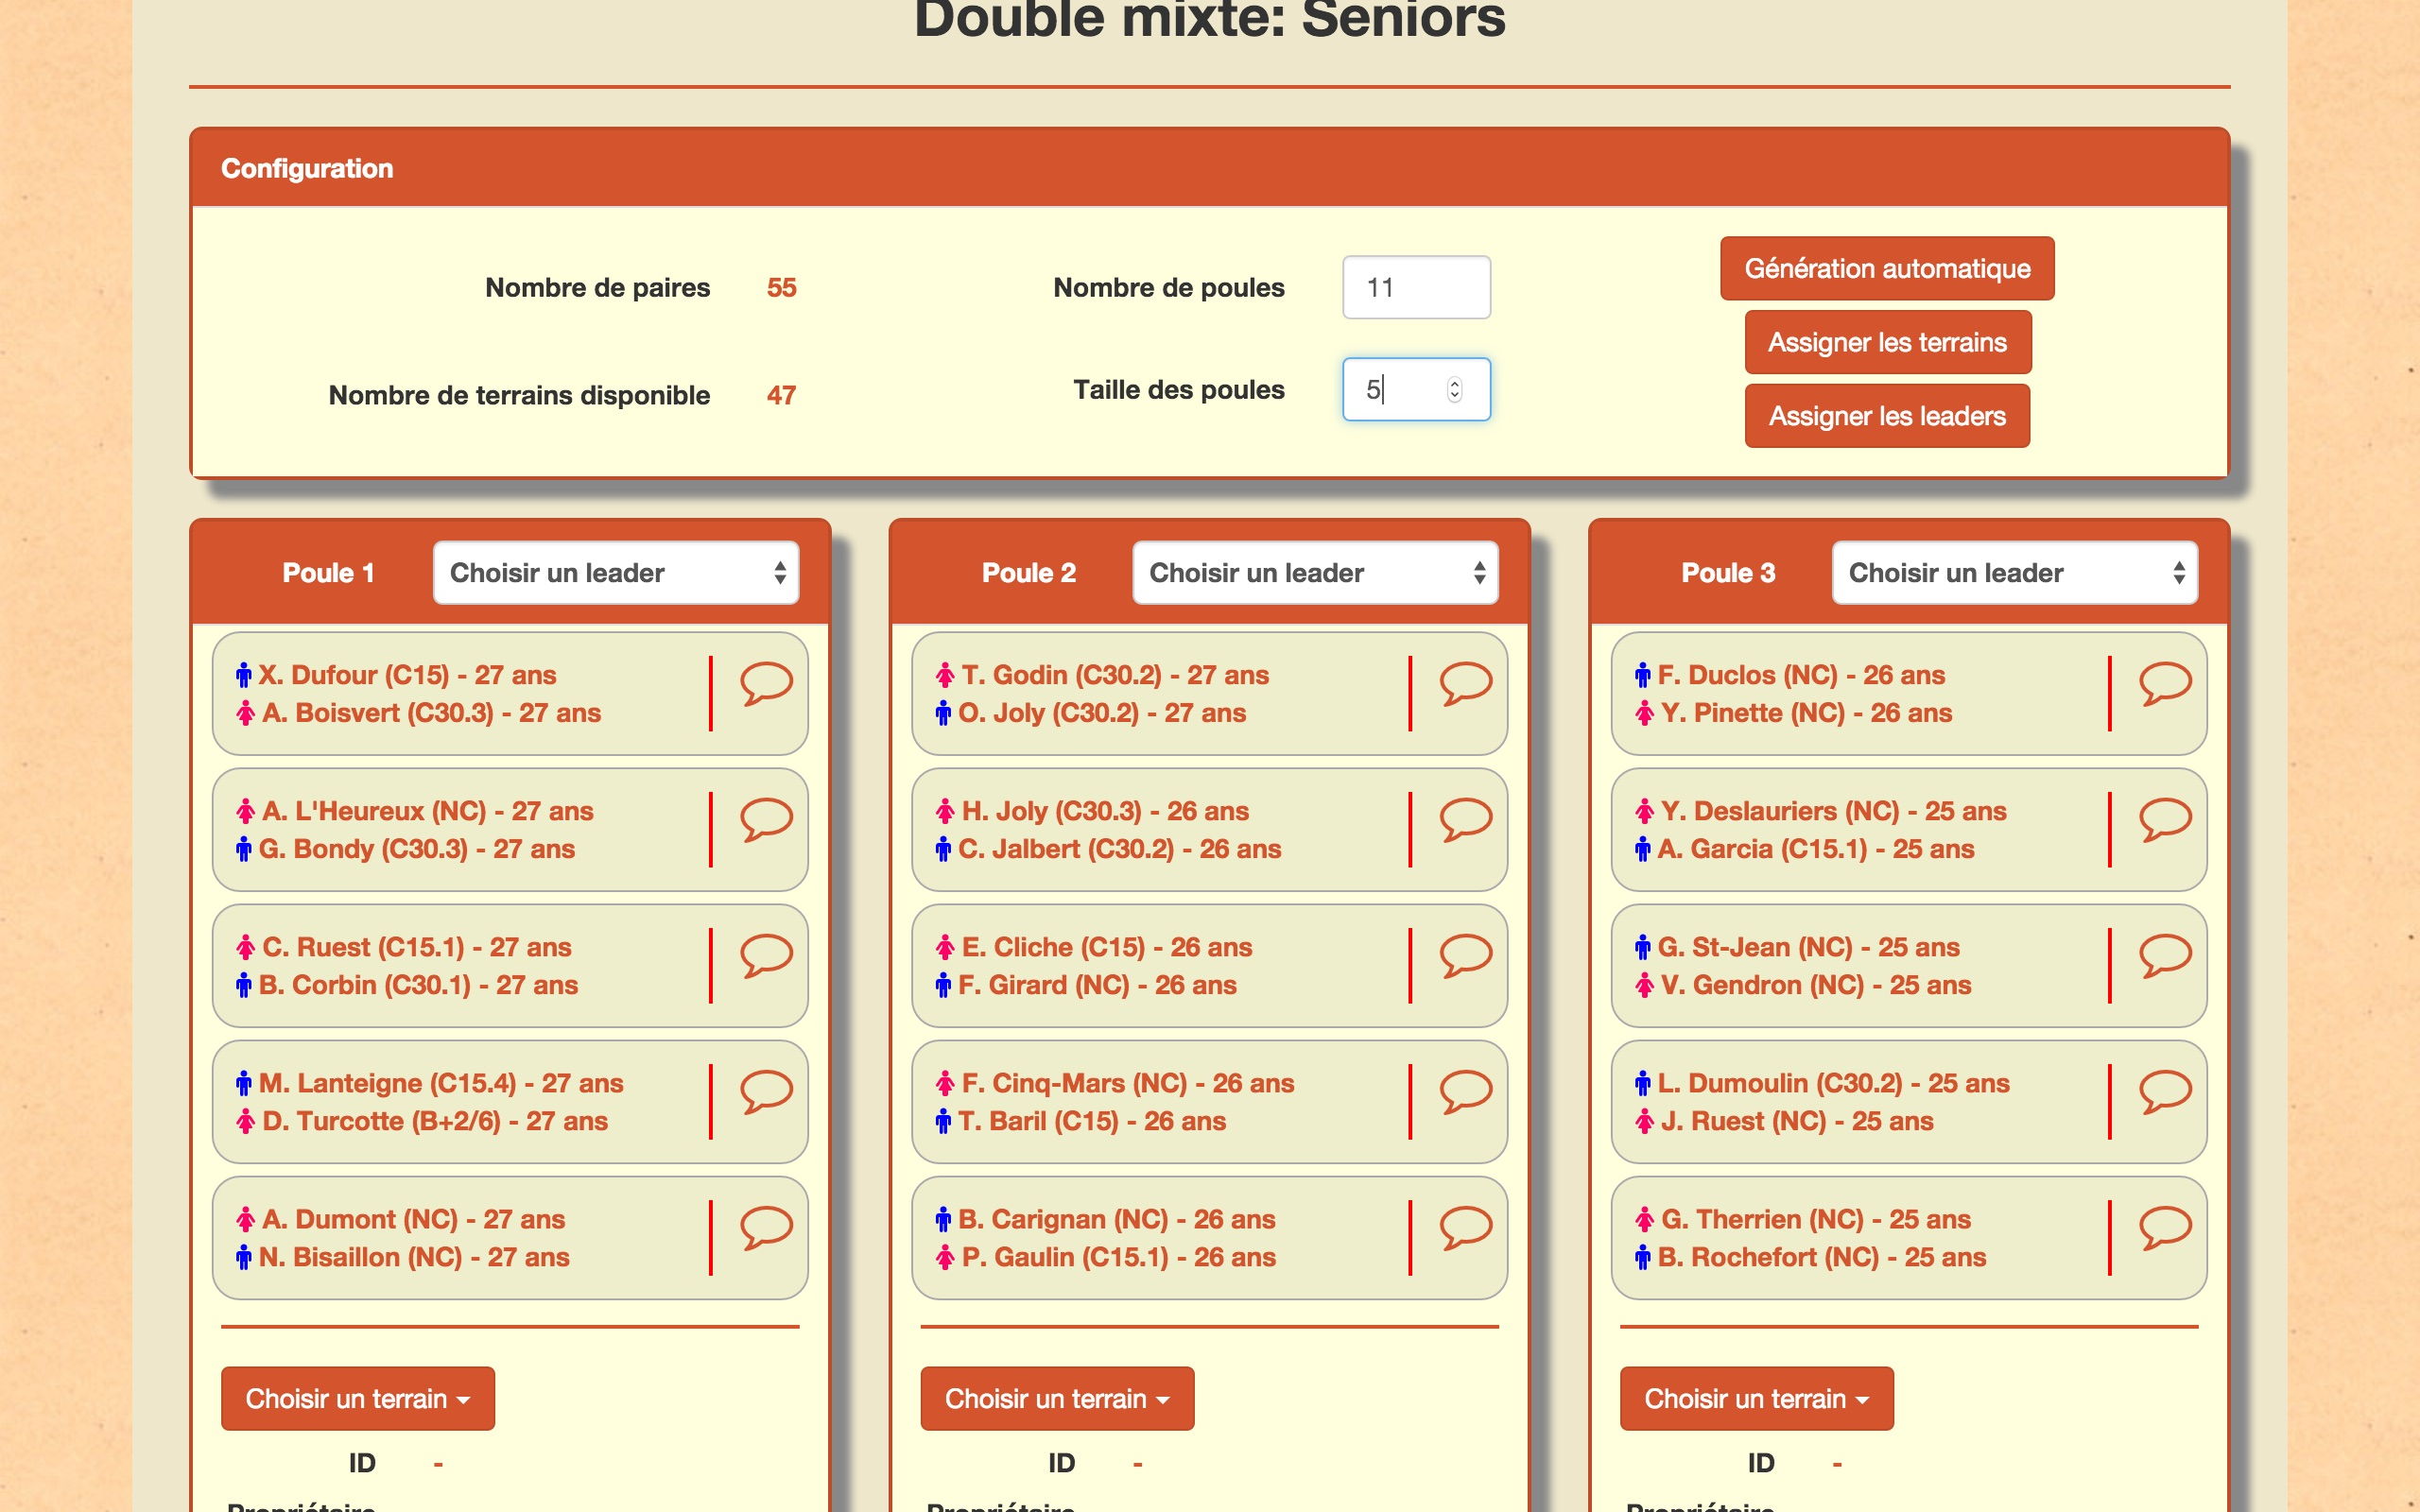
\includegraphics[scale=0.15]{user_images/basic_user/GererTournois/InscriptionComplete/007.jpg}
\caption{Inscription à un tournoi, étape 7}
\end{figure}

L'inscription de la paire est pratiquemment terminée. Il suffit plus qu'un membre du staff valide la paire.

\begin{figure}[H]
\centering
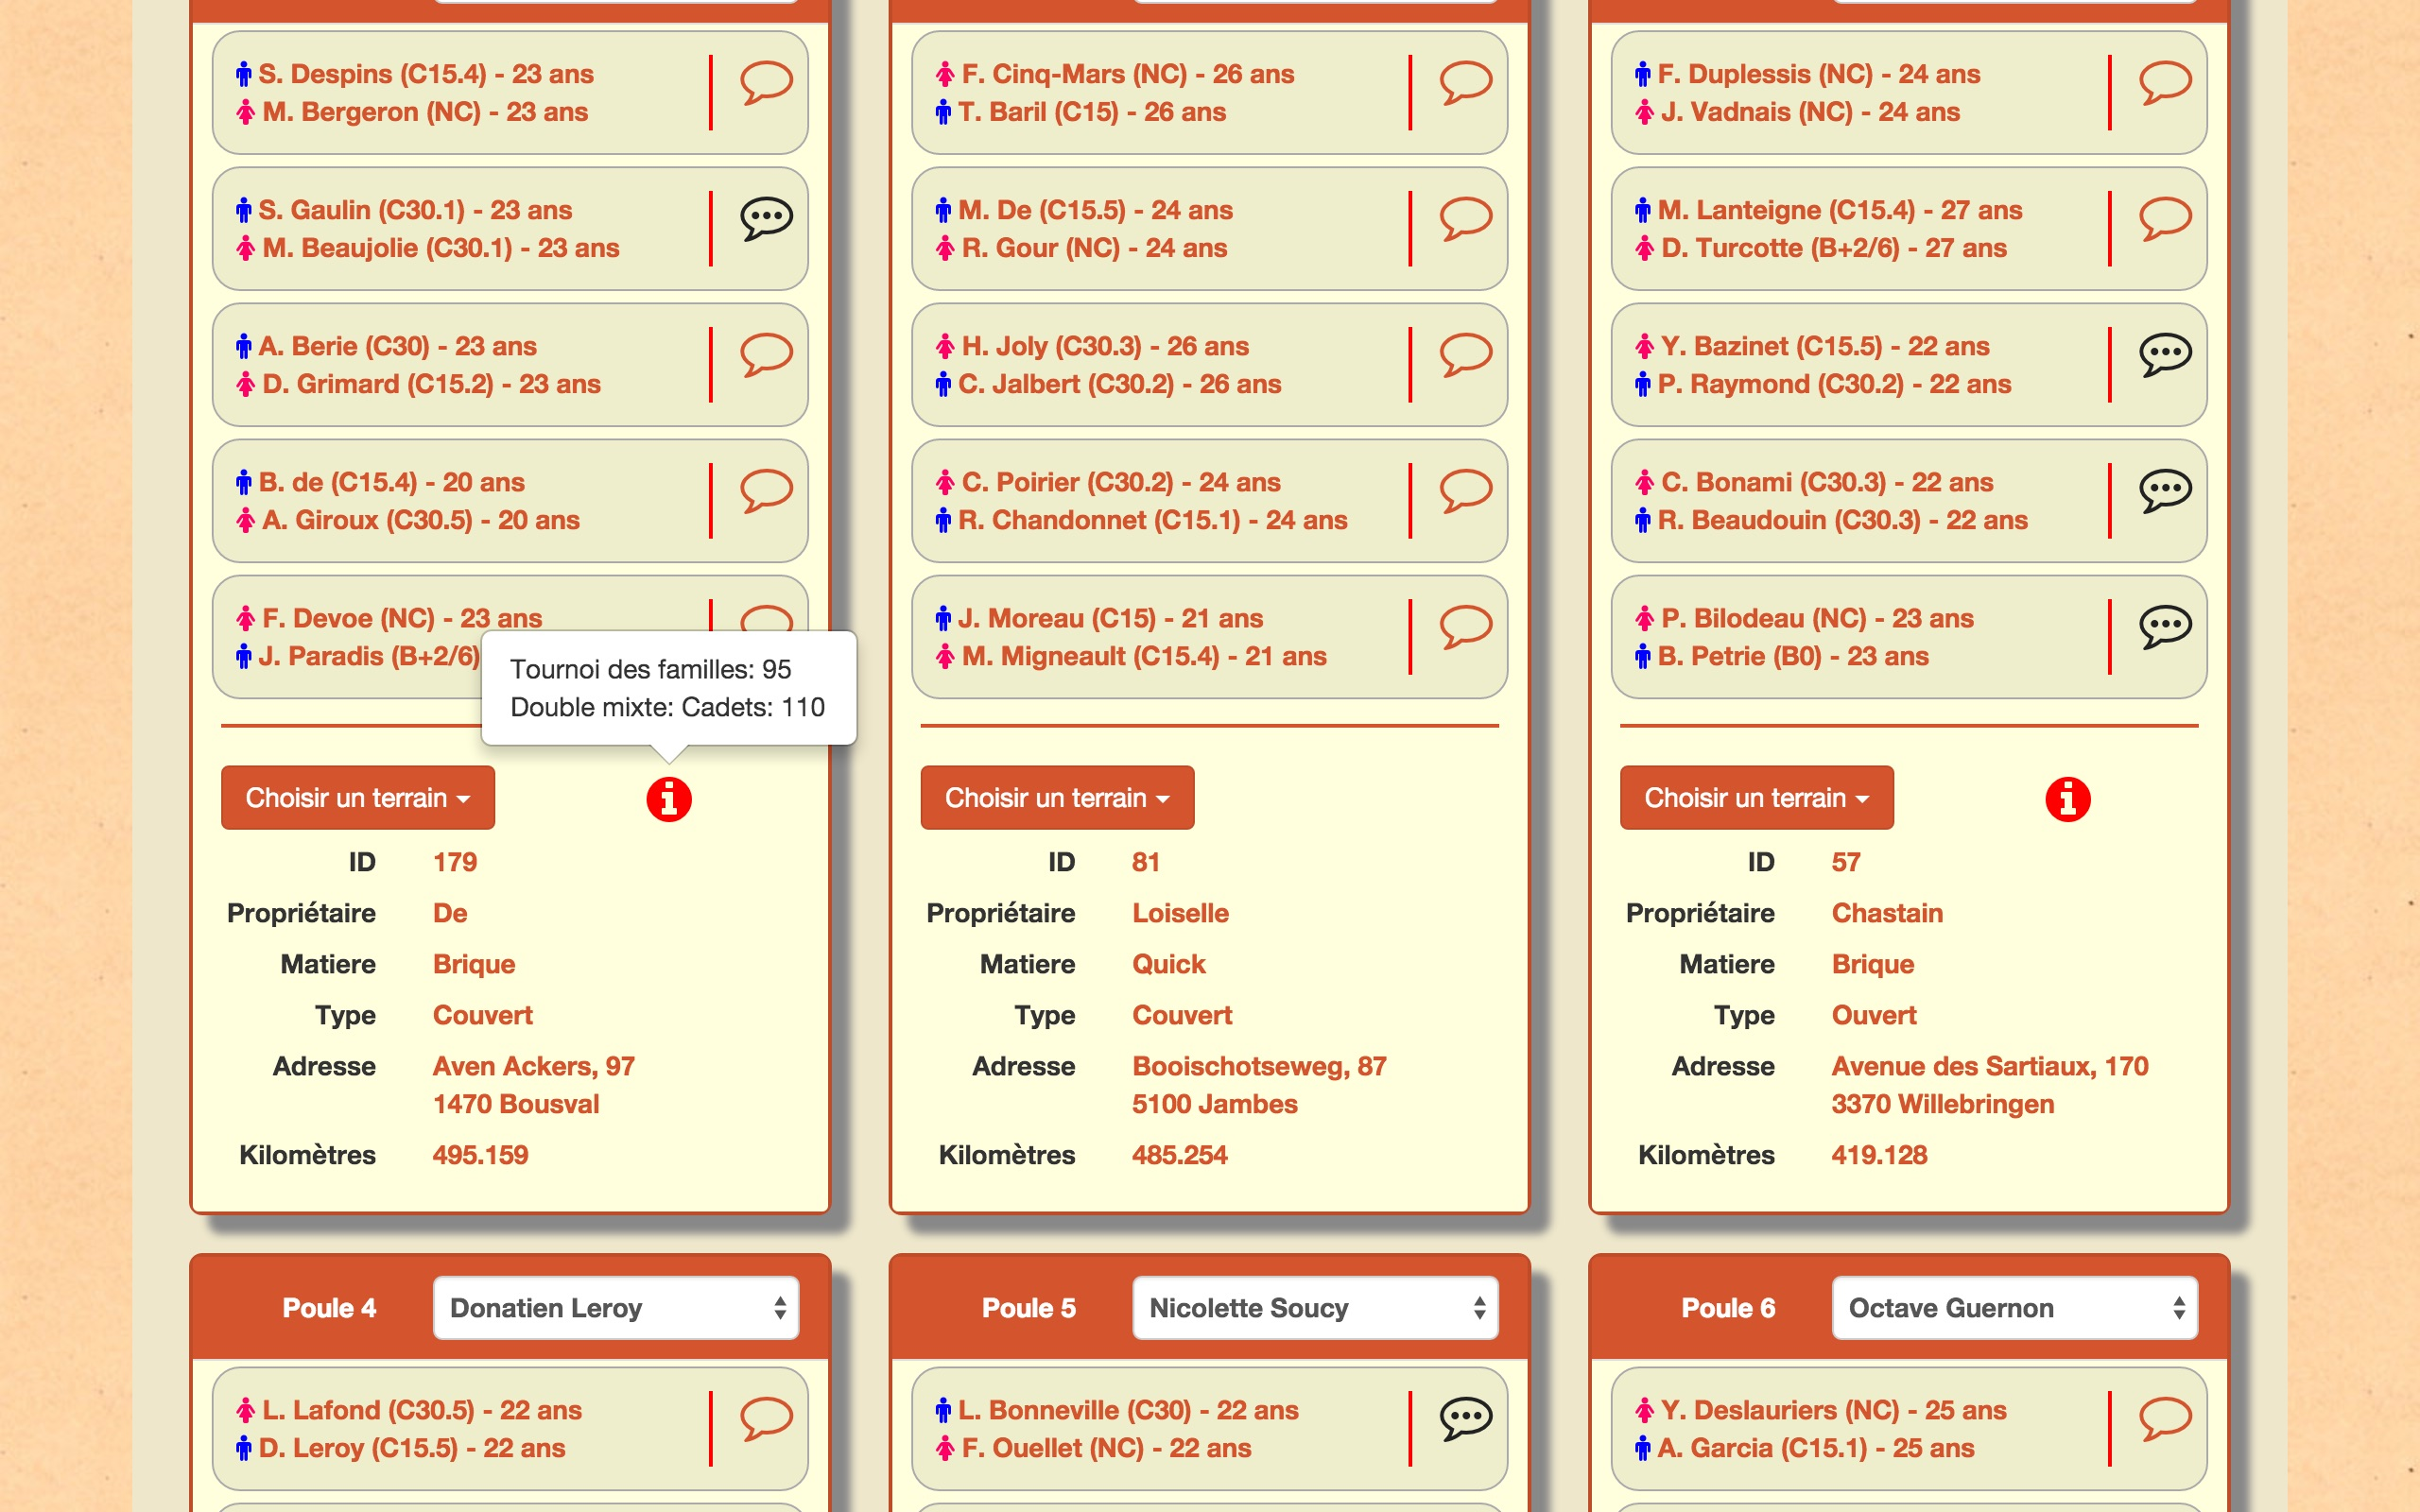
\includegraphics[scale=0.15]{user_images/basic_user/GererTournois/InscriptionComplete/008.jpg}
\caption{Inscription à un tournoi, étape 8}
\end{figure}

Dès qu'un membre du staff a validé la paire, celle-ci participera au tournoi inscrit.

\begin{figure}[H]
\centering
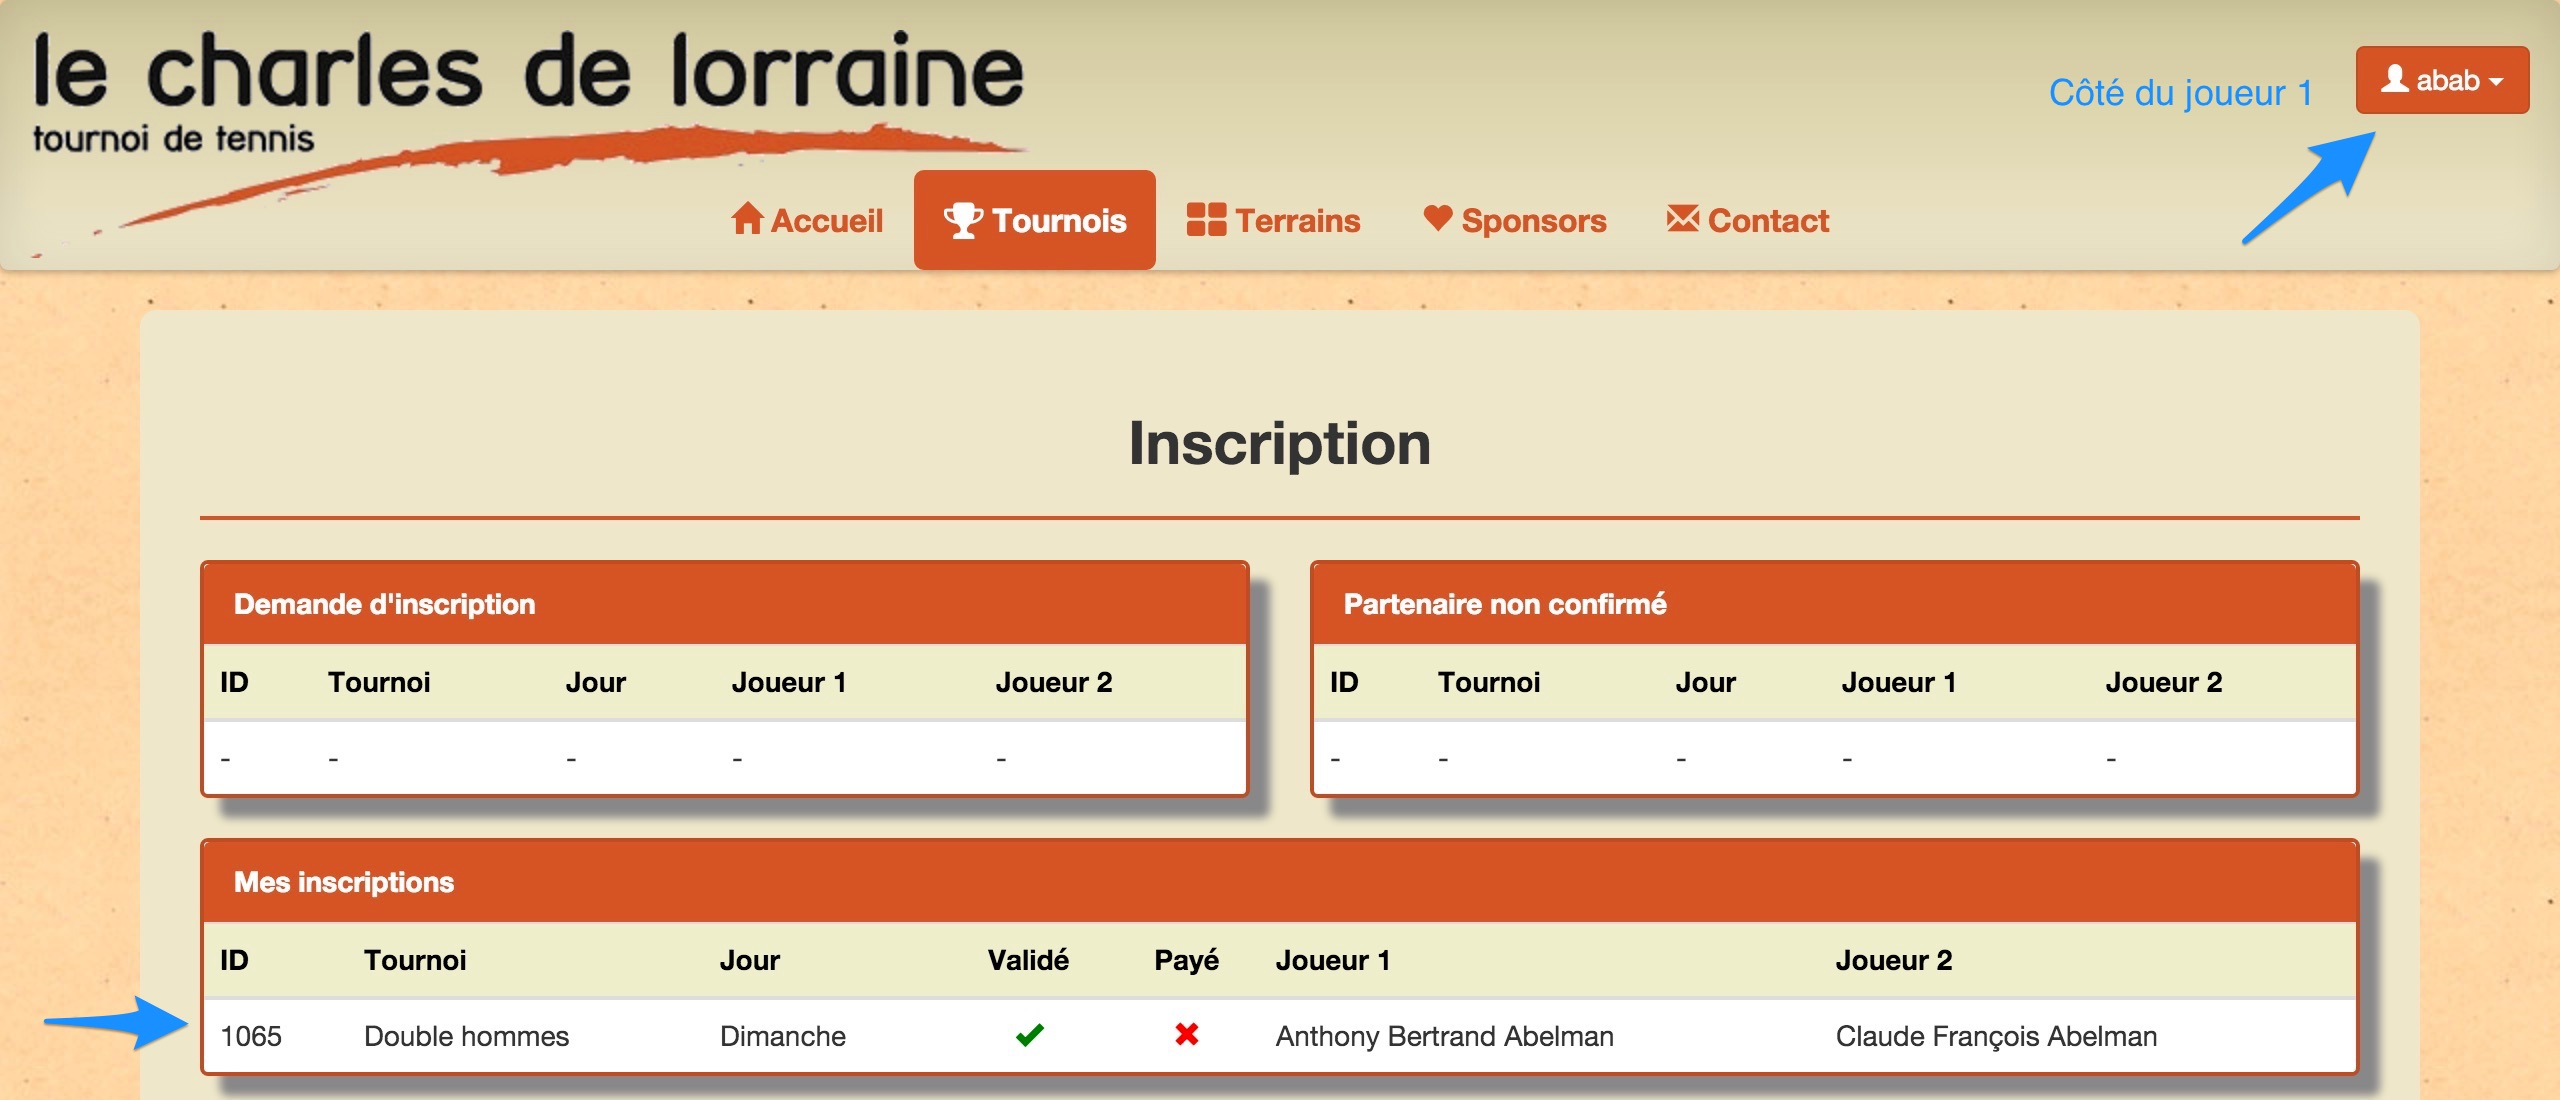
\includegraphics[scale=0.15]{user_images/basic_user/GererTournois/InscriptionComplete/009.jpg}
\caption{Inscription à un tournoi, étape 9}
\end{figure}

\subsection{Annuler inscription à un tournoi}

Il est possible d'annuler l'inscription, par un utilisateur standard, à un tournoi lorsque le deuxième joueur n'a pas accepté l'inscription en paire.\newline

Pour le 1er joueur, il suffit de consulter ses inscriptions en cours de confirmation de la part du 2ème joueur, en cliquant sur la paire temporairement créée dans la liste en haut à droite de la page.

\begin{figure}[H]
\centering
\includegraphics[scale=0.15]{user_images/basic_user/GererTournois/AnnulerInscription/AnnulerDemandeJoueur1/001.jpg}
\caption{Annulation inscription tournoi par joueur 1, étape 1}
\end{figure}

Sur la page de la demande de paire, il est possible d'annuler la demande d'inscription de la paire en cliquant sur le bouton "Supprimer".

\begin{figure}[H]
\centering
\includegraphics[scale=0.15]{user_images/basic_user/GererTournois/AnnulerInscription/AnnulerDemandeJoueur1/002.jpg}
\caption{Annulation inscription tournoi par joueur 1, étape 2}
\end{figure}

Cette action est irréversible. Une boîte de dialogue demande à l'utilisateur de confirmer son choix de suppression de la paire en cours d'inscription.

\begin{figure}[H]
\centering
\includegraphics[scale=0.15]{user_images/basic_user/GererTournois/AnnulerInscription/AnnulerDemandeJoueur1/003.jpg}
\caption{Annulation inscription tournoi par joueur 1, étape 3}
\end{figure}

Si l'utilisateur confirme son souhait d'annuler son inscription, il sera bien désinscrit du tournoi.

\begin{figure}[H]
\centering
\includegraphics[scale=0.15]{user_images/basic_user/GererTournois/AnnulerInscription/AnnulerDemandeJoueur1/004.jpg}
\caption{Annulation inscription tournoi par joueur 1, étape 4}
\end{figure}

Le joueur 2 peut aussi annuler l'inscription à un tournoi en refusant une demande d'inscription. Sur sa page de tournoi, il peut consulter à la demande de confirmation de la paire en cliquant sur la demande souhaitée, en haut à gauche de la page.

\begin{figure}[H]
\centering
\includegraphics[scale=0.15]{user_images/basic_user/GererTournois/AnnulerInscription/AnnulerDemandeJoueur2/001.jpg}
\caption{Annulation inscription tournoi par joueur 2, étape 1}
\end{figure}

Ensuite, au lieu de choisir ses extras, écrire un commentaire, et accepter la demande, celui-ci peut cliquer sur le bouton "Refuser" pour refuser la demande d'inscription au tournoi.

\begin{figure}[H]
\centering
\includegraphics[scale=0.15]{user_images/basic_user/GererTournois/AnnulerInscription/AnnulerDemandeJoueur2/002.jpg}
\caption{Annulation inscription tournoi par joueur 2, étape 2}
\end{figure}

Comme cette action est irréversible, il est demandé à l'utilisateur de confirmer son choix de refuser la demande d'inscription au tournoi.

\begin{figure}[H]
\centering
\includegraphics[scale=0.15]{user_images/basic_user/GererTournois/AnnulerInscription/AnnulerDemandeJoueur2/003.jpg}
\caption{Annulation inscription tournoi par joueur 2, étape 3}
\end{figure}

L'inscription au tournoi sera bien annulé.

\begin{figure}[H]
\centering
\includegraphics[scale=0.15]{user_images/basic_user/GererTournois/AnnulerInscription/AnnulerDemandeJoueur2/004.jpg}
\caption{Annulation inscription tournoi par joueur 2, étape 4}
\end{figure}

\subsection{Payer son inscription}

Pour effectuer le paiement de la paire à l'inscription à un tournoi, l'un des deux joueurs de la paire doit consulter les informations de la paire, en cliquant sur sur l'inscription dans la liste des inscriptions, sur la page "Tournois".

\begin{figure}[H]
\centering
\includegraphics[scale=0.15]{user_images/basic_user/GererTournois/PaiementInscription/001.jpg}
\caption{Paiement inscription au tournoi, étape 1}
\end{figure}

Ensuite, il doit cliquer sur le bouton "Payer", en bas de la page.

\begin{figure}[H]
\centering
\includegraphics[scale=0.15]{user_images/basic_user/GererTournois/PaiementInscription/002.jpg}
\caption{Paiement inscription au tournoi, étape 2}
\end{figure}

Sur cette page, l'utilisateur peut consulter le coût total de l'inscription de la paire, ainsi que choisir le mode de paiement vous payer l'inscription. Plusieurs modes de paiement sont disponibles, comme Visa, Paypal, ou Mastercard.

\begin{figure}[H]
\centering
\includegraphics[scale=0.15]{user_images/basic_user/GererTournois/PaiementInscription/003.jpg}
\caption{Paiement inscription au tournoi, étape 3}
\end{figure}

Lorsque la paire aura payé son inscription, et que le staff aura bien reçu l'information du paiement, un membre du staff indiquera que la paire a bien payée son inscription.

\begin{figure}[H]
\centering
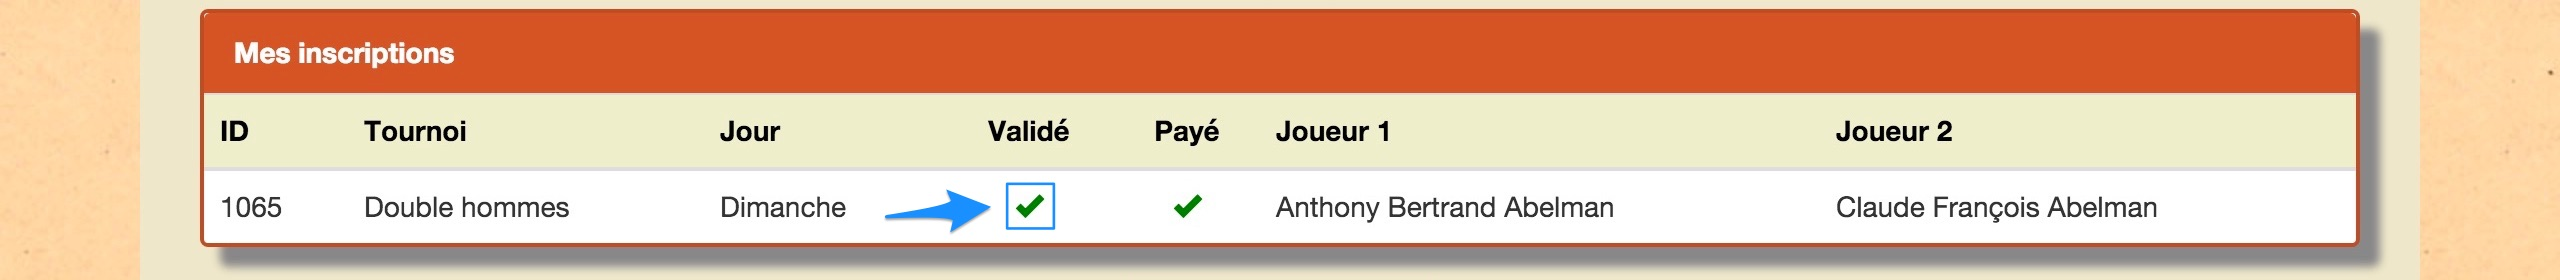
\includegraphics[scale=0.15]{user_images/basic_user/GererTournois/PaiementInscription/au_final.jpg}
\caption{Paiement inscription au tournoi, étape finale}
\end{figure}

\section{La page des terrains}

Vous êtes l'heureux propriétaire d'un terrain de tennis ? C'est par ici !

\subsection{Gérer ses terrains}

\textbf{Si vous n'avez pas de terrains enregistrés}, vous pouvez en ajouter un
en cliquant sur \textit{Enregistrer un nouveau terrain}. Vous serez amené à
compléter un formulaire nous permettant de savoir les disponibilités de votre
terrain ainsi que les informations d'accès utiles à nos joueurs.

\begin{figure}[H]
\centering
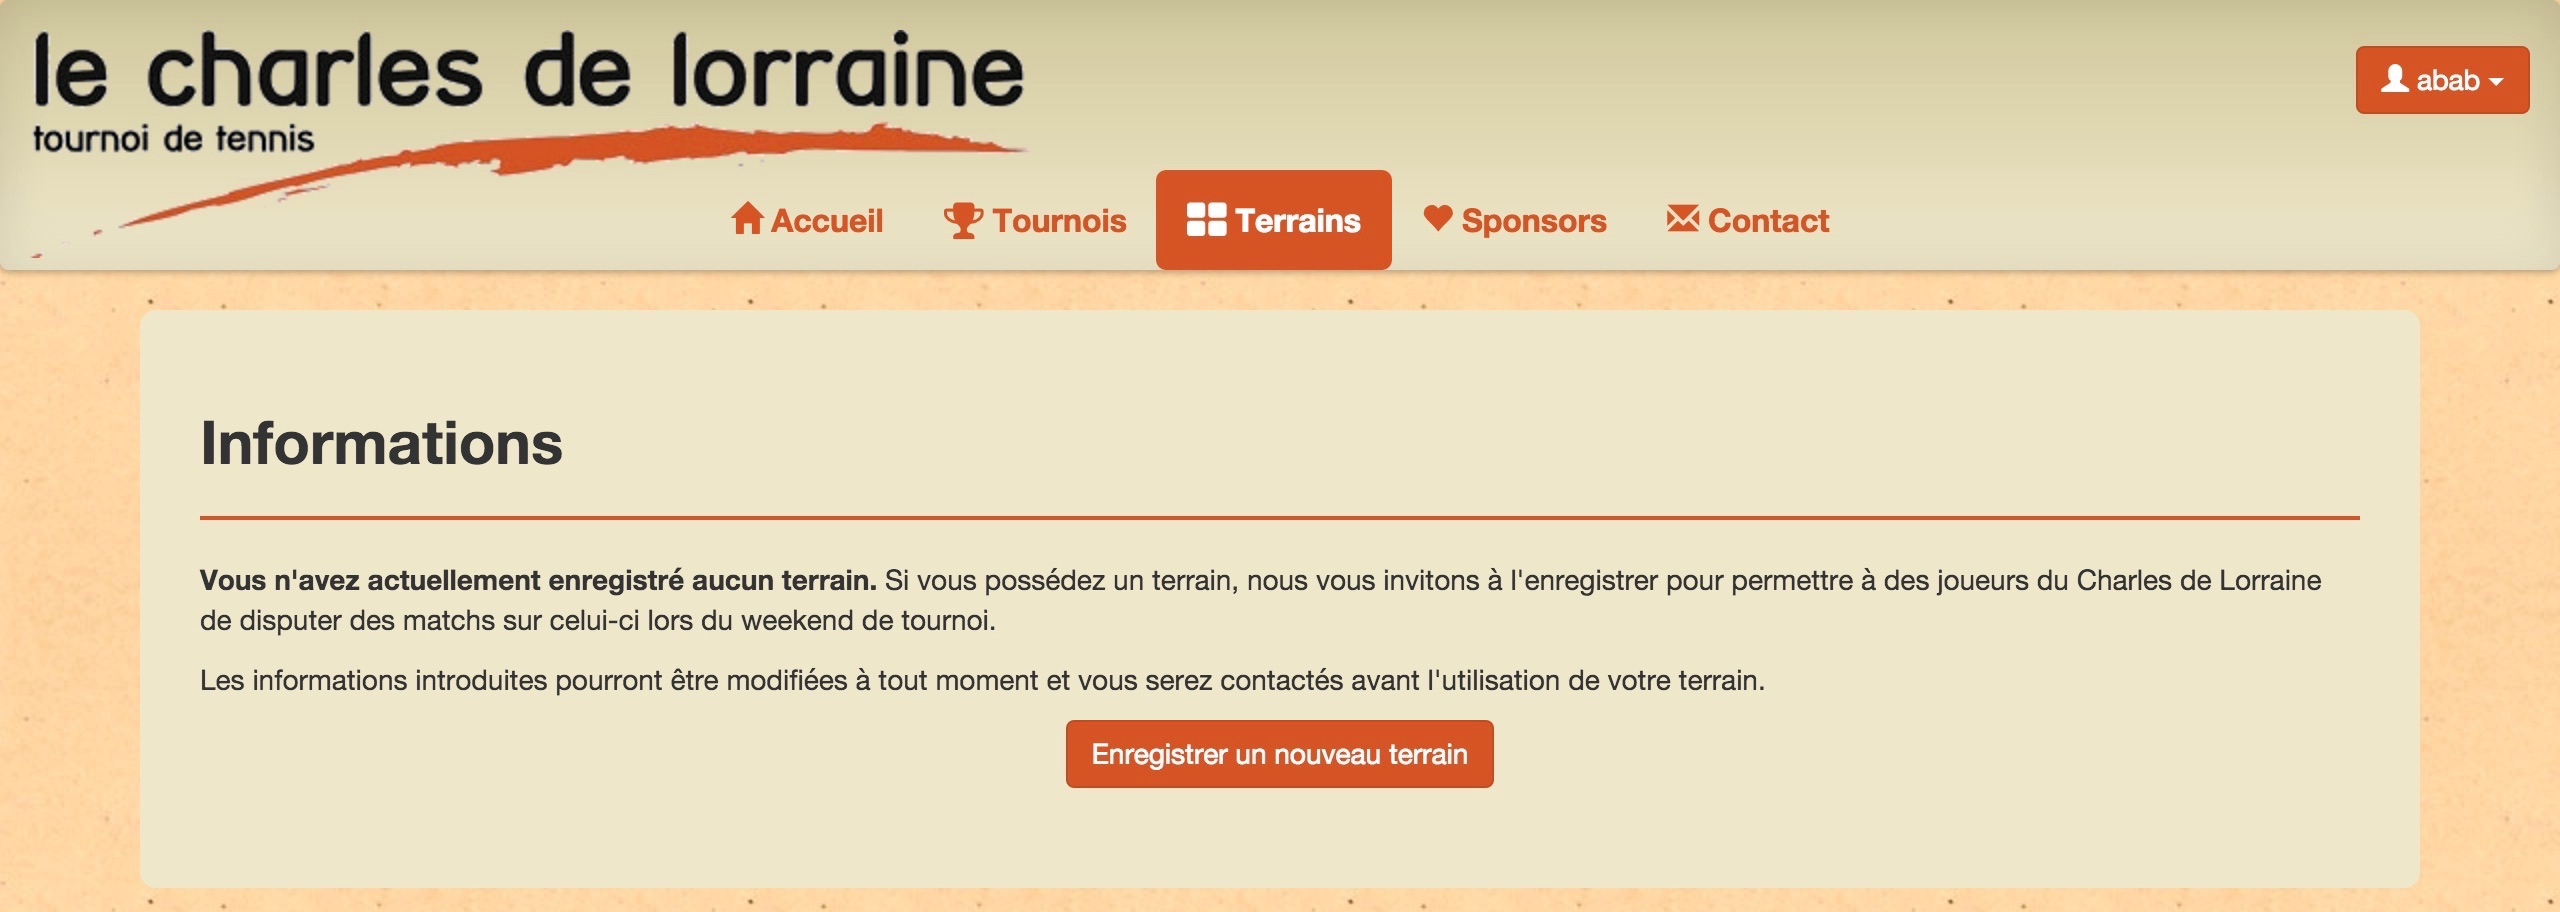
\includegraphics[scale=0.15]{page-terrains/page-terrains-sans.jpg}
\caption{Page des terrains - aucun terrain enregistré}
\end{figure}

\textbf{Si vous avez déjà un terrain enregistré} :

\begin{itemize}
    \item Vous pouvez accéder à ses informations et les modifier en cliquant
    sur le résumé du terrain.
    \item Vous pouvez supprimer votre terrain si vous ne souhaitez plus que
    le Charles de Lorraine puisse l'utiliser. Nous serions ravis si vous
    pouviez au préalable nous en informer via notre formulaire de contact pour
    assurer la bonne gestion du tournoi ;
    % TODO
    \todo[inline]{Ajouter une référence vers le formulaire de contact}
    \item Vous aurez accès aux informations d'utilisation de votre terrain pour
    savoir si votre terrain sera utilisé pour le tournoi. Ces informations
    sont mises à jour lorsque l'équipe aura assigné les joueurs dans les
    tournois ;
    \item Vous pouvez ajouter un terrain supplémentaire en cliquant sur le
    bouton \textit{Enregistrer un nouveau terrain} et vous serez ainsi dirigé
    vers un formulaire identique à celui complété pour le premier terrain.
\end{itemize}

\begin{figure}[H]
\centering
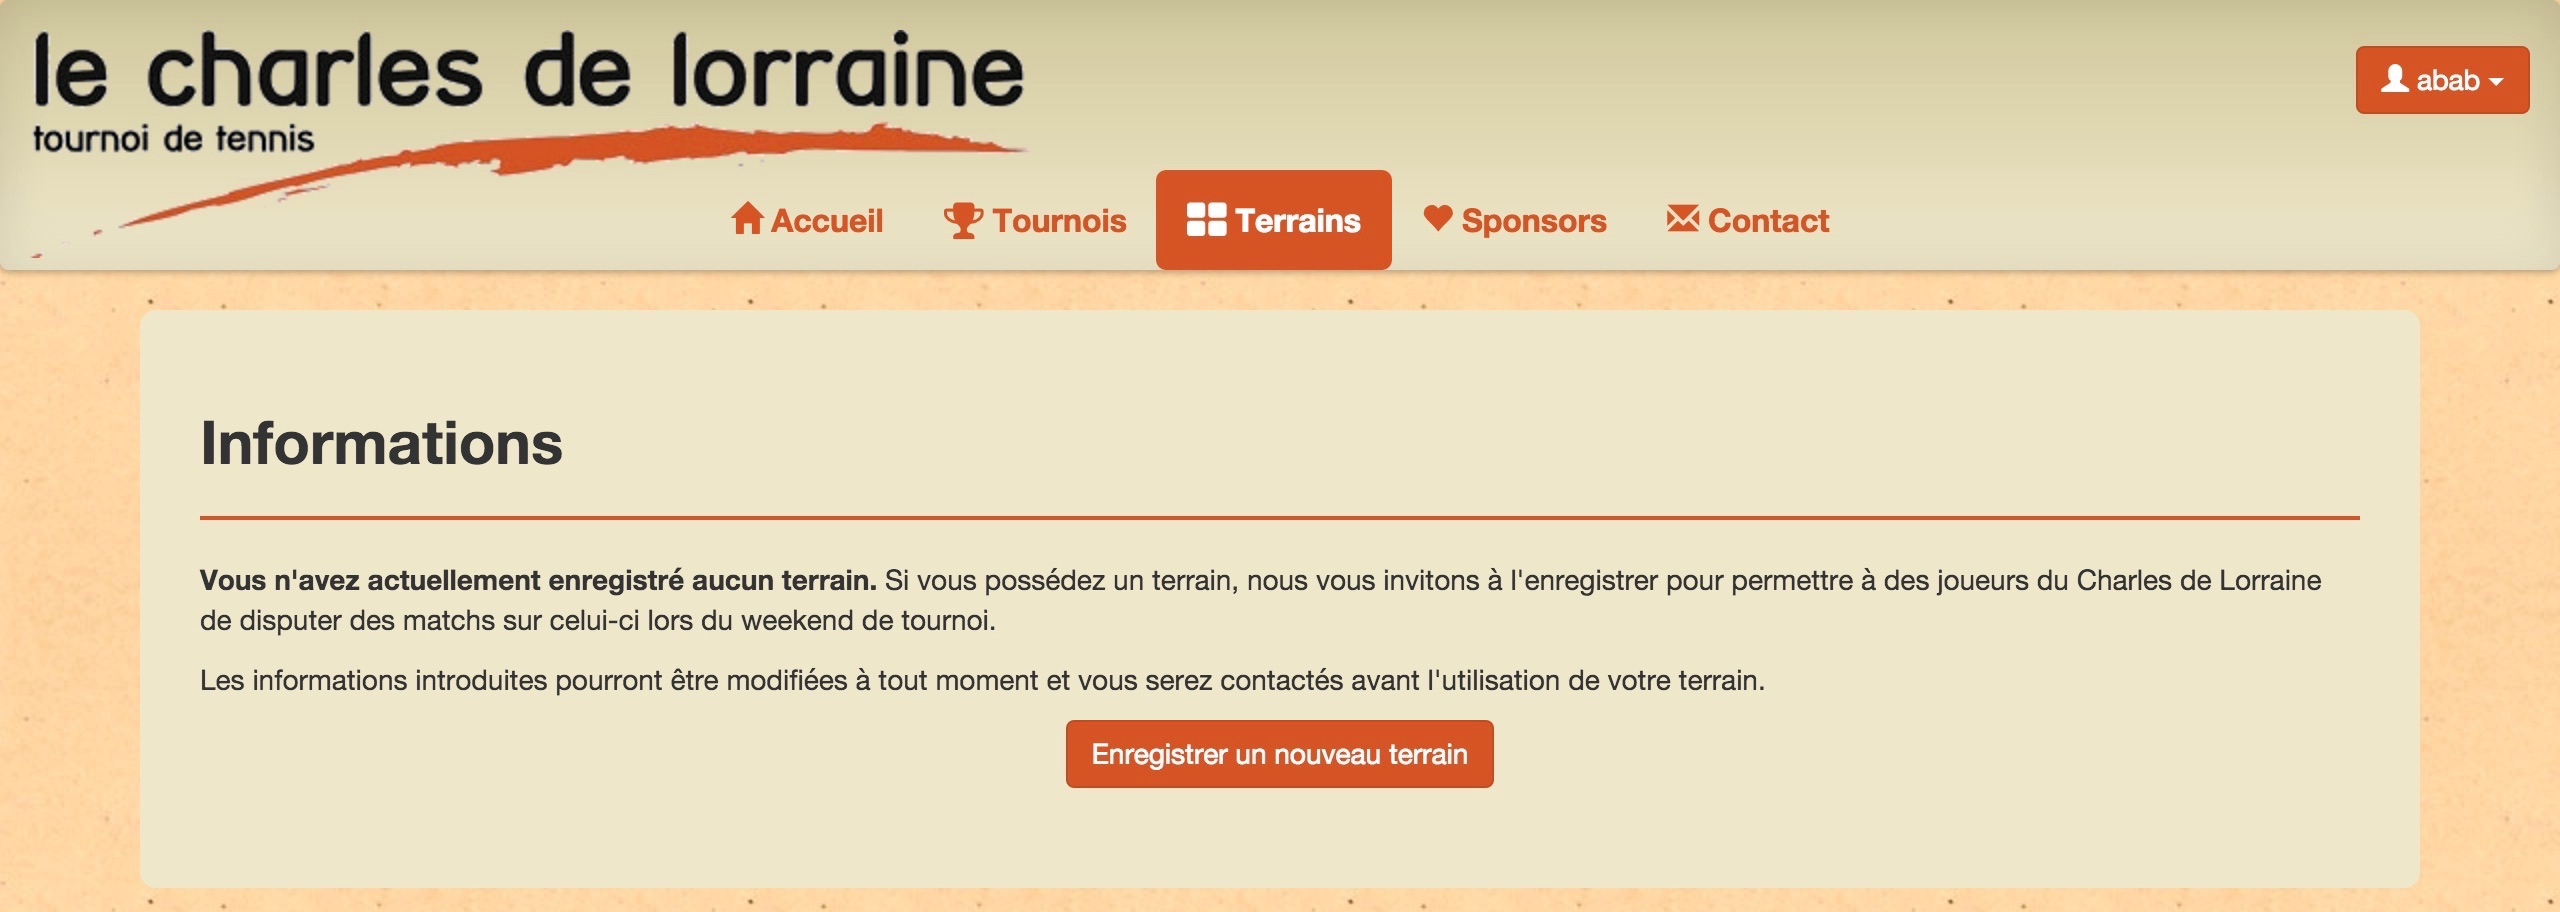
\includegraphics[scale=0.15]{page-terrains/page-terrains-sans.jpg}
\caption{Page des terrains - terrains enregistrés}
\end{figure}


\chapter{Utilisateur staff}

Cette catégorie concerne les utilisateurs staff. Elle décrit les fonctionnalités propre aux membres du staff, qui sont décomposées en plusieurs modules appelés "gestionnaires".

\begin{figure}[H]
\centering
\includegraphics[scale=0.15]{user_images/staff/001.jpg}
\caption{Accès au parties staff du site}
\end{figure}

\section{Gestion des tournois}

\textbf{Si vous êtes membres du staff, et que vous avez la permission de gérer les tournois}, vous pouvez alors accéder à la page de gestion des tournois, depuis l'onglet "Staff" tout à droite du menu de navigation.

\begin{figure}[H]
\centering
\includegraphics[scale=0.15]{gestion-tournois/gestion-tournois.jpg}
\caption{Page de la gestion des tournois}
\end{figure}

\subsection{Les tournois}

Depuis la page staff "Gestionnaire des tournois", vous pouvez gérer tous les tournois et catégories dont vous avez eu préalablement la permission de gérer. Pour donner la permission à un utilisateur de gérer certains tournois, l'admin doit lui octroyer les permission à partir de la page "Gestionnaire des permissions".
% TODO
\todo[inline]{Ajouter une référence vers la page Gestionnaire des permissions}

Sur cette page, vous pouvez consulter une liste de tournois. Les tournois sont catégorisés en fonction du type du tournoi :

\begin{itemize}
\item Tournoi des familles
\item Double mixte
\item Double hommes
\item Double femmes
\end{itemize}

\begin{figure}[H]
\centering
\includegraphics[scale=0.15]{gestion-tournois/gestion-tournois-liste.jpg}
\caption{Page de la gestion des tournois - liste des tournois}
\end{figure}

Tous les tournois, sauf le Tournoi des familles, sont à nouveau catégorisés en fonction de l'âge des joueurs. Ces sous-tournois sont ordonnés du tournoi des plus jeunes (Pré-minimes), au plus âgés (Élites).\newline

Chaque tournois indique les informations les plus importantes, à savoir :

\begin{itemize}
\item le nombre de paires inscrites
\item le nombre de poules actuel
\item le status du tournoi
\end{itemize}
\bigskip

L'état du tournoi impose les opérations possibles sur le tournoi. Par exemple :

\begin{itemize}
\item  \textbf{Aucune poules} n'autorise que de générer les poules ;
\item \textbf{Poules validées} permet d'encoder les scores ;
\item \textbf{Poules terminées} permet de consulter les poules, et de créer l'arbre d'élimination.
\end{itemize}
\bigskip

Il y a 3 boutons d'accès aux pages spécifiques de gestion des tournois, selon le status de celui-ci :

\begin{itemize}
\item \textit{Générer Poules} : permet de créer, modifier, et sauvegarder les poules
\item \textit{Scores} : permet de consulter les poules crées, supprimer les poules, imprimer les score boards, et encoder les scores de chaque poule
\item \textit{Arbre de Tournoi} : permet de créer l'arbre du tournoi, imprimer l'arbre d'élimination, et encoder les scores dans l'arbre d'élimination
\end{itemize}

\begin{figure}[H]
\centering
\includegraphics[scale=0.35]{gestion-tournois/gestion-tournois-operations.jpg}
\caption{Page de la gestion des tournois - accès aux pages spécifique de gestion}
\end{figure}

\subsection{Les poules}

Toutes les fonctionnalités des tournois propres aux poules dépendent du status du tournoi, comme décrit à la section sur la liste des tournois.
% TODO
\todo[inline]{Ajouter une référence vers la section précédente, sur les opérations et boutons selon le status.}
\bigskip

Il existe deux pages pour interagir avec les poules d'un tournoi :

\begin{itemize}
\item \textbf{Création des poules} (Génération des poules)
\item \textbf{Gestion des poules} (Scores)
\end{itemize}

\subsubsection{Création des poules}

La première page des poules d'un tournoi est la création des poules. Elle est accessible à partir de la page "Gestionnaire des tournois", en cliquant sur le bouton du tournoi qui se trouve à la colonne "Générer Poules".

\begin{figure}[H]
\centering
\includegraphics[scale=0.35]{creation-poules/creation-poules-bouton.jpg}
\caption{Bouton d'accès à la page de création des poules}
\end{figure}

Ce bouton est cliquable uniquement pour les status de tournoi suivant:

\begin{itemize}
\item \textbf{Aucune poules} : c'est le status initial d'un tournoi
\item \textbf{Poules sauvegardées} : c'est le status du tournoi lorsque les poules sont en cours de création, mais qu'elles n'ont pas encore totalement validées.
\end{itemize}
\bigskip

La page de création de poules se présente avec un module de configuration de toutes les poules, et plusieurs modules correspondant aux poules du tournoi.

\begin{figure}[H]
\centering
\includegraphics[scale=0.15]{creation-poules/creation-poules.jpg}
\caption{Page de création des poules}
\end{figure}

Le module de configuration des poules permet de connaître le nombre de paires et de terrain disponibles, de définir le nombre et la taille des poules du tournoi, et 3 boutons d'assistance à la création des poules.

\begin{figure}[H]
\centering
\includegraphics[scale=0.15]{creation-poules/creation-poules-configuration.jpg}
\caption{Module de configuration de création des poules}
\end{figure}

En modifiant la taille des poules (respectivement, le nombre de poules), le nombre de poules (respect., la taille des poules) s'adaptent automatiquement pour permettre à toutes les paires d'être dans une poule.\newline

Les boutons d'assistance à la création des poules sont les suivants:

\begin{itemize}
\item \textit{Génération automatique} : ce bouton permet d'assigner automatiquement les paires par poules, les leaders, et les terrains de chacunes des poules.
\item \textit{Assigner les terrains} : ce bouton permet d'assigner automatiquement les terrains de toutes les poules.
\item \textit{Assigner les leaders} : ce bouton permet d'assigner automatiquement les leaders de toutes les poules.
\end{itemize}
\bigskip

Les poules peuvent, à tout moment, être éditées. Un leader peut être assigné à une poule, en sélectionnant un joueur parmi tous les joueurs de la poule. Pour ce faire, sélectionner un joueur dans la liste déroulante en titre du module de la poule.

\begin{figure}[H]
\centering
\includegraphics[scale=0.35]{creation-poules/creation-poules-leader.jpg}
\caption{Sélection du leader d'une poule}
\end{figure}

Le procédé pour assigner manuellement un terrain à une poule est similaire à celui de l'assignation d'un leader, sauf que cette sélection se trouve en bas du module de la poule. En cliquant sur le bouton \textit{Choisir un terrain}, une liste déroulante propose tous les terrains disponibles.

\begin{figure}[H]
\centering
\includegraphics[scale=0.2]{creation-poules/creation-poules-terrain.jpg}
\caption{Sélection d'un terrain d'une poule}
\end{figure}

Dès que le terrain a été sélectionné, les informations du terrain sont résumées, tout en indiquant le nombre de kilomètres total que les joueurs de la poule doivent parcourir au minimum. Si le terrain est déjà en cours d'utilisation dans ce tournoi ou un autre, un petit avertissement en rouge le signale. En cliquant sur ce bouton, on peut savoir rapidement dans quel tounoi ce terrain est déjà utilisé.

\begin{figure}[H]
\centering
\includegraphics[scale=0.4]{creation-poules/creation-poules-avertissement.jpg}
\caption{Avertissement d'un terrain déjà utilisé}
\end{figure}

L'information sur le kilométrage total permet d'estimer l'empreinte carbone de la poule, qui peut être un paramètre que le responsable du tournoi pourrait souhaiter minimiser. Le bouton d'assignation automatique tente de minimiser cette valeur, pour toutes les poules, tout en choisissant pour leader le joueur le plus proche du QG de ASMAE.\newline

Les paires peuvent être manuellement permutées, au sein d'une poule ou entre deux poules différentes, en utilisant deux interactions possibles :

\begin{itemize}
\item la première interaction consiste à faire un \textit{drag-and-drop} d'une case d'une paire vers une autre case d'une autre paire. C'est interaction a l'avantage d'être intuitive.
\item la deuxième interaction consiste à faire un \textit{click-and-drop} d'une case d'une paire vers une autre case d'une autre paire. Cette interaction a l'avantage d'être facilement réalisable, même avec un nombre et des tailles de poules élevés.
\end{itemize}

\begin{figure}[H]
\centering
\includegraphics[scale=0.25]{creation-poules/creation-poules-dragndrop.jpg}
\caption{Interaction \textit{drag-and-drop} pour permuter deux paires}
\end{figure}

Il est aussi possible de créer les poules en prenant en compte les remarques et souhaits des paires. Chaque paire possède une icône de de bulle de dialogue à sa droite. Les bulles vides indiquent que la paire n'a aucune remarques ou commentaires, tandis que les bulles avec trois points sont des paires ayant des commentaires. En passant le curseur sur une bulle remplie, les commentaires de la paire s'affiche à l'écran.

\begin{figure}[H]
\centering
\includegraphics[scale=0.45]{creation-poules/creation-poules-commentaire.jpg}
\caption{Commentaire d'une paire}
\end{figure}

Si l'on souhaite enregistrer l'état actuel de la création des poules, on peut cliquer sur le bouton \textit{Sauvegarder} en bas de la page. Dès que toutes les poules ont des leaders et terrains assignés, il est possible de finaliser la création des poules, en cliquant sur le bouton \textit{Valider}. Si des terrains ont des avertissements, la boîte de dialogue demande clairement à l'utilisateur de confirmer la validation des poules, malgré les conflits sur les terrains.

\subsubsection{Gestion des poules}

La deuxième page des poules d'un tournoi est la gestion des poules. Elle est accessible à partir de la page "Gestionnaire des tournois", en cliquant sur le bouton du tournoi qui se trouve à la colonne "Scores".

\begin{figure}[H]
\centering
\includegraphics[scale=0.45]{gestion-poules/gestion-poules-bouton.jpg}
\caption{Bouton d'accès à la gestion des poules}
\end{figure}

Ce bouton est cliquable uniquement pour les status de tournoi suivant:

\begin{itemize}
\item \textbf{Poules validées} : c'est le status du tournoi lorsque les poules ont été totalement créées et validéés, prêtes pour imprimer les score boards et encoder les scores.
\item \textbf{Poules terminées} : c'est le status du tournoi lorsque toutes les poules ont été encodées, et donc la création de l'arbre d'élimination peut commencer
\end{itemize}

La page de gestion des poules se présente avec un module par poule.

\begin{figure}[H]
\centering
\includegraphics[scale=0.15]{gestion-poules/gestion-poules.jpg}
\caption{Page de gestion des poules d'un tournoi}
\end{figure}

Chaque poule contient le nombre de paires, la liste de toutes les paires, le leader, et le terrain assigné. Il est possible d'obtenir le scoreboard de la poule, en cliquant sur bouton dans le coin droit supérieur du module, avec une icône d'imprimante.

\begin{figure}[H]
\centering
\includegraphics[scale=0.3]{gestion-poules/gestion-poules-poule.jpg}
\caption{Module d'une poule de la page de gestion des poules}
\end{figure}

Il est possible d'encoder les scores des matchs de la poules en cliquant sur le bouton \textit{Entrer les scores}. Ce bouton permet d'accéder à un score board interactif. Les scores doivent être entrés dans les champs, où le premier champ de la case est le nombre de points de la paire sur la ligne, et le deuxième champ est le nombre de points de la paire sur la colonne. Les scores sont symétriques par rapport à la diagonale : par exemple, le score à la première ligne, deuxième colonne est à tout moment l'inverse du score à la deuxième ligne, première colonne du score board.

\begin{figure}[H]
\centering
\includegraphics[scale=0.15]{gestion-poules/gestion-poules-score.jpg}
\caption{Page du score board interactif de la poule}
\end{figure}

Le score board interactif peut être enregistré, ou valider pour afficher définitivement les scores de la poule. Lorsque les scores sont validés, les scores totaux de la poule sont résumés sur la page de gestion des poules.

\begin{figure}[H]
\centering
\includegraphics[scale=0.3]{gestion-poules/gestion-poules-encode.jpg}
\caption{Module d'une poule encodées dans la page de gestion des poules du tournoi}
\end{figure}

En bas de la page de la gestion des poules, il est possible de télécharger les score boards de toutes les poules à la fois en cliquant sur le bouton \textit{Version PDF}. Il est également possible de supprimer toutes les poules, et revenir à l'étape de "Poules sauvegardées" du tournoi, en cliquant sur le bouton \textit{Supprimer les poules}. Enfin, le bouton \textit{Arbre de Tournoi} permet d'accéder à la page de l'arbre d'élimination, uniquement accessible lorsque toutes les poules ont été encodées.

\subsection{L'arbre d'élimination}

Toutes les fonctionnalités des tournois propres aux arbres sont accessibles uniquement aux tournois dont le status sont l'un des deux suivants :

\begin{itemize}
\item \textbf{Poules terminées} : lorsque toutes les poules ont été encodées, et l'arbre d'élimination n'a pas été créé ou est non terminé (c'est-à-dire qu'il n'y a pas encore de gagnant)
\item \textbf{Tournoi terminé} : lorsque l'arbre d'élimination a été complètement encodé, et qu'il y a un gagnant du tournoi
\end{itemize}
\bigskip

Il y a une seule page spécifique à l'arbre d'élimination du tournoi, qui s'adapte automatiquement à 2 cas différents :

\begin{itemize}
\item Toutes les poules ont étés encodées, et aucun arbre d'élimination n'a été créé (Création de l'arbre).
\item Toutes les poules ont été encodées, et un arbre d'élimination a été créé et enregistré (Gestion de l'arbre)
\end{itemize}
\bigskip

Cette page est accessible de deux manières différentes :

\begin{itemize}
\item soit par la page principale de "Gestionnaire des poules, en cliquant sur le bouton sous la colonne "Arbre de tournoi".
\item soit par la page de gestion des poules, lorsque toutes les poules ont été encodées, en cliquant sur le bouton \textit{Arbre du tournoi} en bas de page.
\end{itemize}
\bigskip

\begin{figure}[H]
\centering
\includegraphics[scale=0.45]{creation-arbre/creation-arbre-bouton.jpg}
\caption{Accés à la page de l'arbre d'élimination, depuis la page principale de la gestion des tournois}
\end{figure}

\subsubsection{Création de l'arbre}

Si aucun arbre d'élimination n'a été préalablement enregistré, ou bien que toutes les poules ont été récemment encodées, alors les deux accès à la page de l'arbre d'élimination est accessible. En accédant à la page de l'arbre du tournoi, puisqu'aucun arbre n'a encore été créé, il est demandé à l'utilisateur de choisir les paires sélectionnées pour le tournoi d'élimination.

\begin{figure}[H]
\centering
\includegraphics[scale=0.15]{creation-arbre/creation-arbre-etape1.jpg}
\caption{Première étape de la création d'un arbre - sélection des paires}
\end{figure}

Les paires sont triées par leurs points totaux au sein d'une poule, de la paire aux points les plus élevés jusqu'à la paire aux points les moins élevés. Les scores sont affichés entre parenthèses à côté des noms des joueurs de la paire. L'icône à droite de la case d'une paire indique si la paire est sélectionnée ou non pour l'arbre d'élimination. Pour modifier l'état de sélection de la paire, il faut cliquer sur la case de la paire.\newline

Dès que les paires cochées sont celles que l'on souhaite avoir pour commencer l'arbre d'élimination, on peut poursuivre le processus de création de l'arbre d'élimination en cliquant sur le bouton \textit{Prochaine étape}, tout en bas de la page.\newline

Sur cette deuxième et dernière page de création de l'arbre, il est demandé de choisir un terrain et l'ordre des paires au départ de l'arbre. Ces deux paramètres sont divisés en deux modules différents :

\begin{itemize}
\item Le module "Terrain" permet d'assigner un terrain, de la même manière que lors de la création des poules : soit manuellement en cliquant sur le bouton \textit{Choisir un terrain}, soit automatiquement en cliquant sur le bouton \textit{Assigner Terrain}.
\item Le module "Premier Round", qui permet d'ordonner les paires au début de l'arbre d'élimination, en interagissant avec \textit{drag-and-drop}.
\end{itemize}
\bigskip

Pour ordonner efficacement les paires au départ de l'arbre d'élimination, l'identifiant de la poule et la position dans la poule (ordonné selon le score total) est précisé pour chacune des paires.

\begin{figure}[H]
\centering
\includegraphics[scale=0.3]{creation-arbre/creation-arbre-etape2.jpg}
\caption{Deuxième et dernière étape de la création de l'arbre - sélection du terrain et ordre des paires}
\end{figure}

Pour finaliser le processus de création de l'arbre, il suffit de cliquer sur le bouton \textit{Voir l'arbre du tournoi}, en bas de la page. N'oubliez pas d'enregistrer l'arbre dès que l'arbre a été créé, sinon vous devez recommencer le processus de création de l'arbre ! Pour enregistrer l'arbre créé, cliquez simplement sur le bouton Enregistrer en bas de la page de gestion de l'arbre d'élimination


\subsubsection{Gestion de l'arbre}

Si un arbre d'élimination a été enregistré, alors la page de l'arbre d'élimination du tournoi permettra d'accéder directement à la page avec l'arbre interactif du tournoi.

\begin{figure}[H]
\centering
\includegraphics[scale=0.15]{gestion-arbre/gestion-arbre.jpg}
\caption{Page de gestion de l'arbre d'élimination}
\end{figure}

Cette page est divisée en deux parties :

\begin{itemize}
\item la première partie contient un module interactif d'encodage de l'arbre d'élimination.
\item La deuxième partie contient un module d'information sur le terrain du tournoi d'élimination, avec les boutons de gestion de l'arbre en bas de la page.
\end{itemize}
\bigskip

L'arbre d'élimination donne une représentation de l'arbre du tournoi, où chaque case est une paire. Deux cases verticalement collée entre elles représentent le match des deux paires, l'une contre l'autre.

\begin{figure}[H]
\centering
\includegraphics[scale=0.5]{gestion-arbre/gestion-arbre-match.jpg}
\caption{Match entre deux paires dans l'arbre d'élimination interactif}
\end{figure}

Pour encoder le score d'un match, il suffit de cliquer sur l'une des deux paires, et d'inscrire le score du match dans la boîte de dialogue. Ensuite, le gagnant sera automatiquement placé à l'étape suivante de l'arbre d'élimination. N'oubliez pas d'enregistrer l'arbre d'élimination après avoir encodé les scores, sinon l'arbre n'est pas mise à jour !\newline

Lorsque l'arbre d'élimination est complètement encodée, c'est-à-dire lorsqu'il y a un gagnant dans le tournoi, et que l'arbre est enregistrée, alors le status du tournoi devient "Tournoi terminé".\newline

En plus du bouton \textit{Enregistrer}, qui permet d'enregistrer l'état de l'arbre d'élimination, deux autres boutons se trouve en bas de la page:

\begin{itemize}
\item \textit{Version PDF} : permet d'imprimer l'arbre du tournoi et l'information du terrain.
\item \textit{Enregistrer} : permet d'enregistrer l'état de l'arbre du tournoi.
\item \textit{Supprimer} : permet de supprimer l'arbre d'élimination, et de revenir à l'étape de création de l'arbre d'élimination.
\end{itemize}
\bigskip

\section{Gestion des terrains}


\section{Gestion des paires}

\subsection{Les paires}

\section{Gestionnaire des utilisateurs}

Cette section décrit comment gérer les utilisateurs par un membre du staff. Pour accéder à cette page, l'utilisateur doit avoir la permission de gérer les utilisateurs (voir la section "Gestionnaire des permissions").\newline

Le gestionnaire des utilisateur permet de gérer les utilisateurs. En particulier, il est possible de modifier les informations d'un utilisateur.

\begin{figure}[H]
\centering
\includegraphics[scale=0.15]{user_images/staff/GererUtilisateurs/001.jpg}
\caption{Gestionnaire des utilisateurs}
\end{figure}

Cette page est divisée en deux parties: à droite, une liste des utilisateurs, à gauche, des critères de recherche pour affiner la liste des utilisateurs à droite. En bas à gauche, il est possible d'exporter la liste des utilisateurs au format CSV, ou bien uniquement la liste des adresses (toujours au format CSV).

\subsection{Consulter un utilisateur}

Pour consulter à un utilisateur, il faut cliquer sur l'entrée de la liste des utilisateurs à droite de l'écran correspondant à cet utilisateur.

\begin{figure}[H]
\centering
\includegraphics[scale=0.15]{user_images/staff/GererUtilisateurs/ConsulterUtilisateur/001.jpg}
\caption{Consulter un utilisateur, étape 1}
\end{figure}

On accède ensuite à la page de l'utilisateur, qui reprend les informations du joueurs, ainsi que les tournois inscrits et les terrains possédés.

\begin{figure}[H]
\centering
\includegraphics[scale=0.15]{user_images/staff/GererUtilisateurs/ConsulterUtilisateur/002.jpg}
\caption{Consulter un utilisateur, étape 2}
\end{figure}

\subsection{Editer un utilisateur}

Pour éditer un utilisateur, il faut accéder à la page de cet utilisateur, comme expliqué précédemment dans la sous-section "Consulter un utilisateur".

À partir de la page de l'utilisateur à éditer, cliquez sur le bouton "Modifier informations" pour accéder à la modification des informations de l'utilisateur.

\begin{figure}[H]
\centering
\includegraphics[scale=0.15]{user_images/staff/GererUtilisateurs/ModifierUtilisateur/001.jpg}
\caption{Editer un utilisateur, étape 1}
\end{figure}

Une boîte de dialogue, assez complexe, contient un formulaire pré-rempli des informations actuelles de l'utilisateur. Les champs indiqués par une étoile (*) sont obligatoires, et ne peuvent pas être vides.

\begin{figure}[H]
\centering
\includegraphics[scale=0.15]{user_images/staff/GererUtilisateurs/ModifierUtilisateur/002.jpg}
\caption{Editer un utilisateur, étape 2}
\end{figure}

Après avoir modifiés certains champs, comme ici le GSM, le numéro, et le classement, cliquez sur le bouton "Sauver" pour valider les modifications.

\begin{figure}[H]
\centering
\includegraphics[scale=0.15]{user_images/staff/GererUtilisateurs/ModifierUtilisateur/003.jpg}
\caption{Editer un utilisateur, étape 3}
\end{figure}

Après avoir appliqué les modifications des informations de l'utilisateur, un message vert signale la bonne modification des informations de l'utilisateur.

\begin{figure}[H]
\centering
\includegraphics[scale=0.15]{user_images/staff/GererUtilisateurs/ModifierUtilisateur/004.jpg}
\caption{Editer un utilisateur, étape 4}
\end{figure}

En bas de la page de l'utilisateur, l'historique des modifications sur l'utilisateur confirme, à nouveau, que l'utilisateur a été récemment modifié.

\begin{figure}[H]
\centering
\includegraphics[scale=0.15]{user_images/staff/GererUtilisateurs/ModifierUtilisateur/005.jpg}
\caption{Editer un utilisateur, étape 5}
\end{figure}


\section{Gestion des extras}


\section{Historique des modifications}

\textbf{Si vous êtes un membre du staff}, vous pouvez alors accéder à la page des historiques des modifications, depuis l'onglet \enquote{Staff} tout à droite du menu de navigation.

\begin{figure}[H]
\centering
\includegraphics[scale=0.15]{historique-modifs/historique-modifs.jpg}
\caption{Page staff de l'historique des modifications}
\end{figure}

Cette page est accessible par tous les membres du staff, c'est-à-dire n'importe quel utilisateur qui possède au moins la permission d'accéder à une page staff, depuis l'onglet \enquote{Staff} du menu de navigation.\newline

L'historique des modifications permet de rechercher et consulter les modifications effectuées par tous les membres du staff. Les entrées dans l'historique des modifications n'affichent qu'un résumé des récentes actions du staff : il n'y a aucune d'interaction ou redirection vers les pages ayant été modifiées.\newline

Toutes les autres pages staff ont un historique des 15 dernières modifications effectuées au sein de la page considérée. Par exemple, pour la page de gestion des inscriptions, il y a un historique des dernières modifications effectuées par les membres du staff au niveau de l'inscription. Celui-ci est accessible tout en bas de la page considéré.

\begin{figure}[H]
\centering
\includegraphics[scale=0.15]{historique-modifs/historique-modifs-inscription.jpg}
\caption{Historique des dernières modifications tout en bas de la page de gestion des inscriptions}
\end{figure}

\section{Gestionnaire des permissions}

Cette section décrit les actions de la page gestionnaire des permissions. Cette page n'est accessible qu'aux membre du staff qui sont admin.\newline

Cette page contient, à gauche, une liste des utilisateurs. À droite, l'utilisateur sélectionné y est affiché, avec des cases indiquant les permissions actuelles de cet utilisateur.

\begin{figure}[H]
\centering
\includegraphics[scale=0.15]{user_images/staff/GererPermissions/001.jpg}
\caption{Gestionnaire des permissions}
\end{figure}

\subsection{Modifier les permissions d'un utilisateur}

Pour modifier les permission d'un utilisateur, il suffit d'abord de le sélectionner dans la liste des utilisateurs à gauche de la page.\newline

En sélectionnant un utilisateur (par exemple, le compte abab), et en cochant la case admin, l'utilisateur aura les droit admin dès qu'on aura cliqué sur le bouton "Valider".

\begin{figure}[H]
\centering
\includegraphics[scale=0.15]{user_images/staff/GererPermissions/002.jpg}
\caption{Ajout des permissions complet de staff à un utilisateur}
\end{figure}

Après validation des nouveaux droits de l'utilisateur abab, l'historique des modifications concernant les permissions indique clairement cette modification récente.

\begin{figure}[H]
\centering
\includegraphics[scale=0.15]{user_images/staff/GererPermissions/003.jpg}
\caption{Permissions admin bien ajoutées}
\end{figure}

En se connectant avec l'utilisateur abab, on peut remarquer que toutes les pages staffs sont accessibles, alors qu'elles ne l'étaient avant l'octroi des droits admin.

\begin{figure}[H]
\centering
\includegraphics[scale=0.15]{user_images/staff/GererPermissions/004.jpg}
\caption{Accès aux partie staffs}
\end{figure}